\documentclass[sigconf,edbt]{acmart-edbt2019}

\usepackage{booktabs} % For formal tables
\usepackage{subfigure}
\usepackage{color}
\usepackage{amsmath}
\usepackage{graphicx}
\usepackage{caption}

\usepackage{caption}
\usepackage{color}
\usepackage[ruled]{algorithm}
\usepackage{algorithmic}

\newcommand{\ie}[0]{\textit{i.e.}}
\newcommand{\eg}[0]{\textit{e.g.}}
\newcommand{\etal}[0]{\textit{et al.}}
\newcommand{\wrt}[0]{\textit{w.r.t.}}


\newcommand{\keobf}{\textit{$(k,\epsilon)$-obf}}
\newcommand{\argmin}{\operatornamewithlimits{argmin}}
\newcommand{\genobf}{\texttt{\textbf{genObf}}}
\newcommand{\ere}{$\mathcal{E}RR-$eval}
\newcommand{\pg}{\mathcal{G}}
\newcommand{\Constraint}{$\mathcal{C}$}
\newcommand{\Number}{\|v\|}

\theoremstyle{plain}
\newtheorem{problem}{Problem}
\newtheorem{observation}{Observation}

\newcommand{\methodName}{Squid}
\newcommand{\capMethodName}{SQUID}
\newcommand{\soaName}{Obf}


% Copyright
\setcopyright{rightsretained}

% DOI
\acmDOI{}

% ISBN
\acmISBN{XXX-X-XXXXX-XXX-X}

%Conference
\acmConference[EDBT 2019]{22nd International Conference on Extending Database Technology (EDBT)}{March 26-29, 2019}{Lisbon, Portugal} 
\acmYear{2019}

\settopmatter{printacmref=false, printccs=false, printfolios=false}

\pagestyle{empty} % removes running headers


\begin{document}
\title{SIG Proceedings Paper in LaTeX Format}
\titlenote{Produces the permission block, and copyright information}
\subtitle{Extended Abstract}
\subtitlenote{The full version of the author's guide is available as
  \texttt{acmart.pdf} document}
  

\author{Ben Trovato}
\authornote{Dr.~Trovato insisted his name be first.}
\orcid{1234-5678-9012}
\affiliation{%
  \institution{Institute for Clarity in Documentation}
  \streetaddress{P.O. Box 1212}
  \city{Dublin} 
  \state{Ohio} 
  \postcode{43017-6221}
}
\email{trovato@corporation.com}

\author{G.K.M. Tobin}
\authornote{The secretary disavows any knowledge of this author's actions.}
\affiliation{%
  \institution{Institute for Clarity in Documentation}
  \streetaddress{P.O. Box 1212}
  \city{Dublin} 
  \state{Ohio} 
  \postcode{43017-6221}
}
\email{webmaster@marysville-ohio.com}

\author{Lars Th{\o}rv{\"a}ld}
\authornote{This author is the
  one who did all the really hard work.}
\affiliation{%
  \institution{The Th{\o}rv{\"a}ld Group}
  \streetaddress{1 Th{\o}rv{\"a}ld Circle}
  \city{Hekla} 
  \country{Iceland}}
\email{larst@affiliation.org}

\author{Valerie B\'eranger}
\affiliation{%
  \institution{Inria Paris-Rocquencourt}
  \city{Rocquencourt}
  \country{France}
}
\author{Aparna Patel} 
\affiliation{%
 \institution{Rajiv Gandhi University}
 \streetaddress{Rono-Hills}
 \city{Doimukh} 
 \state{Arunachal Pradesh}
 \country{India}}
\author{Huifen Chan}
\affiliation{%
  \institution{Tsinghua University}
  \streetaddress{30 Shuangqing Rd}
  \city{Haidian Qu} 
  \state{Beijing Shi}
  \country{China}
}

\author{Charles Palmer}
\affiliation{%
  \institution{Palmer Research Laboratories}
  \streetaddress{8600 Datapoint Drive}
  \city{San Antonio}
  \state{Texas} 
  \postcode{78229}}
\email{cpalmer@prl.com}

\author{John Smith}
\affiliation{\institution{The Th{\o}rv{\"a}ld Group}}
\email{jsmith@affiliation.org}

\author{Julius P.~Kumquat}
\affiliation{\institution{The Kumquat Consortium}}
\email{jpkumquat@consortium.net}

% The default list of authors is too long for headers}
% \renewcommand{\shortauthors}{B. Trovato et al.}
\renewcommand{\shortauthors}{}


\begin{abstract}
Graphs in many real-world applications, such as social networks and business to business networks, are not deterministic but uncertain. Research in areas such as social science and viral marketing requires open access to these uncertain graphs, but publishing these datasets often risks exposing sensitive and private data. Current works mainly concentrate on privacy issues with deterministic graphs. The uncertain scenario is overlooked. 

In this paper, we study the problem of publishing uncertain graphs under the syntactic anonymity guarantee. We first demonstrate the limitations of conventional methods in the uncertain scenario. By disregarding the possible world semantics of uncertain graphs, they significantly disrupt the stochastic structure. We develop a syntactically private algorithm, Squid. Squid integrates the possible world semantics into the core of the anonymization. It enables a fine-grained, uncertainty-aware control over the injected noise in a novel way. We apply our method to real uncertain graphs and show its efficiency and practical utility.
\end{abstract}

%
% % The code below should be generated by the tool at
% % http://dl.acm.org/ccs.cfm
% % Please copy and paste the code instead of the example below. 
% %
% \begin{CCSXML}
% <ccs2012>
%  <concept>
%   <concept_id>10010520.10010553.10010562</concept_id>
%   <concept_desc>Computer systems organization~Embedded systems</concept_desc>
%   <concept_significance>500</concept_significance>
%  </concept>
%  <concept>
%   <concept_id>10010520.10010575.10010755</concept_id>
%   <concept_desc>Computer systems organization~Redundancy</concept_desc>
%   <concept_significance>300</concept_significance>
%  </concept>
%  <concept>
%   <concept_id>10010520.10010553.10010554</concept_id>
%   <concept_desc>Computer systems organization~Robotics</concept_desc>
%   <concept_significance>100</concept_significance>
%  </concept>
%  <concept>
%   <concept_id>10003033.10003083.10003095</concept_id>
%   <concept_desc>Networks~Network reliability</concept_desc>
%   <concept_significance>100</concept_significance>
%  </concept>
% </ccs2012>  
% \end{CCSXML}
% 
% \ccsdesc[500]{Computer systems organization~Embedded systems}
% \ccsdesc[300]{Computer systems organization~Redundancy}
% \ccsdesc{Computer systems organization~Robotics}
% \ccsdesc[100]{Networks~Network reliability}


% \keywords{ACM proceedings, \LaTeX, text tagging}


\maketitle

\section{Introduction}

\label{sec:Intro}
Graph privacy issues are becoming increasingly important for many applications such as business to business, social networks and instant-messaging networks. 
This is evidenced by the fact the responsible management of sensitive personal information is explicitly mandated through regulations such as European Union's General Data Protection Regulation.
% There are public concerns on how data companies collect personal information and make it available to marketers. 
Users are afraid that the sensitive personal information can be exploited in harmful ways (e.g., cyberstalking).
Meanwhile, data companies have strong fears of violating privacy regulations. 
Accordingly, there has 
been considerable interest in publishing graph data or analysis result under certain privacy guarantees~\cite{Liu_Towards_2008,Wang2011,Liu_Privacy_2009,Nguyen_Anonymizing_2015,Sala_Sharing_2011,Xiao_Differentially_2014,lee2011}. 
However, the majority of works has been limited to the deterministic scenario. 

In some applications, the graph may be probabilistic by nature. 
For example, in social networks, an edge between two individuals corresponds to an interaction or the influence that is predicted through machine learning models characterized by some level of uncertainty, which can thus be conveniently presented as the probability of the existence of that edge~\cite{Adar_Managing_2007,Kempe_Maximizing_2003}. In these situations, the problem of privacy protection becomes far challenging. 

\textbf{Uncertainty: critical privacy factors}~~First, edge uncertainty contains sensitive information about individuals such as a user's influence in a community or over another individual. 
For example, if we consider a small community, the members and the link structures of the members are known to any participant who is also a member of the community. However, the edge uncertainty such as the ``trustworthiness" of user A to user B should be private.
Second, the extra release of edge uncertainty makes the user identity more vulnerable. 
For example, if we consider a small community, several ``trustworthiness" connections between members are known to an intruder who is also a member of the community. The intruder can match the released probabilistic graph with known information, and serves in privacy attacks.  

\textbf{Uncertainty: critical utility factors} Meanwhile, these probabilistic graph are valuable for research and applications such as marketing and advertising, friend recommendation and modeling the structure and dynamic where uncertainty plays a indispensable role. For example, effective advertising needs to leverage the trust and influence relationships among users (uncertainty) as they may greatly impact users' behavior, as illustrated in Figure~\ref{fig:motivationExample}.  The primitive of these applications is to categorize and compute reachability between any two nodes. Therefore, it is these properties of edge uncertainty that must be preserved. 

\textbf{The limitation of existing methods}~~
In these situation, existing solutions for privacy protection graph publication and analysis do not apply because of the ignorance of edge uncertainty. 

Together, it calls for fundamental anonymization primitives for publishing uncertain graphs which, as ever-argued, would become different from the deterministic ones.

\textbf{Challenge} 
The challenges in privacy-preserving uncertain graph publishing are both semantics and computation driven. 

\textbf{What to xxxx}
% From the perspective of the semantics, there is no privacy notation and utility loss metrics over the probabilistic scenario.   First, it is much more challenging to model attacks where the background knowledge and released data both are probabilistic. 
% Second, it is much more challenging to model the utility loss over 


\textbf{How to anonymize uncertain graph efficiently ?}~~While many graph anonymization algorithms such as k-automorphism are intrinsically hard problems, even the simplest degree anonymization by  contractions with minimal loss of information is known to be NP-hard in the deterministic cases~\cite{}. In the probabilistic scenario, edge modifications are no longer limited to edge addition and deletions but can be infinite probability deviation,hence, more expensive over uncertain graphs. Therefore, exact computation is infeasible with today's large-scale graph data. 
Meanwhile, approximation methods designed for deterministic graphs does not guarantee efficiency and in uncertain graphs. For example, xx xx  

\textbf{Our contribution} In this paper we develop novel strategies for sanitizing uncertain graph with dynamic sampling, and filtering strategies. 
One key idea is that Squid captures the structure
of the original decentralized graph, by incrementally identifying
and refining clusters of connected nodes under local differential
privacy. 
To do so, Squid iteratively xxx.
After obtaining such node clusters, it applies a graph
generation model that utilizes such groups to generate a representative
synthetic social graph. Also, we describe techniques to
optimize critical parameters of xxx to improve the utility of the
generated synthetic social graph.


To validate the effectiveness of Squid, we present an extensive
set of experiments using three real uncertain graphs in various
domains, and two different use cases: (i) statistical analysis of the
 graph structure, (ii) influence propagation. 
 
The experiment results show that synthetic
 generated using Squid obtains high utility for all
use cases and datasets, whereas baseline solutions fail to capture
competitive utility in most settings except for the few that they are
specifically optimized for. 

Our main contributions are summarized as follows: 
\begin{itemize}
\item We formulate the problem of synthetic data generation of uncertain graph under syntactic anonymity while keeping the data utility in mind. To this end, we propose a reliability-driven utility loss metric, which evaluates the connectivity difference in the context of the entire graph and also utilizes the possible world model.  

\item We propose Squid, a novel and effective randomized algorithm to synthetic uncertain graph generation and describe methods for scaling computation. Boosted by the hybrid of uncertainty-aware heuristics, it excels in identifying a population of synthetic results with good quality efficiently. 

\item We conduct a comprehensive experimental study using several
real datasets and use cases. The results demonstrate that
Squid improves the utility of
obtained result, while providing users with their desired privacy guarantees. 
\end{itemize}

\begin{figure}
    \centering
    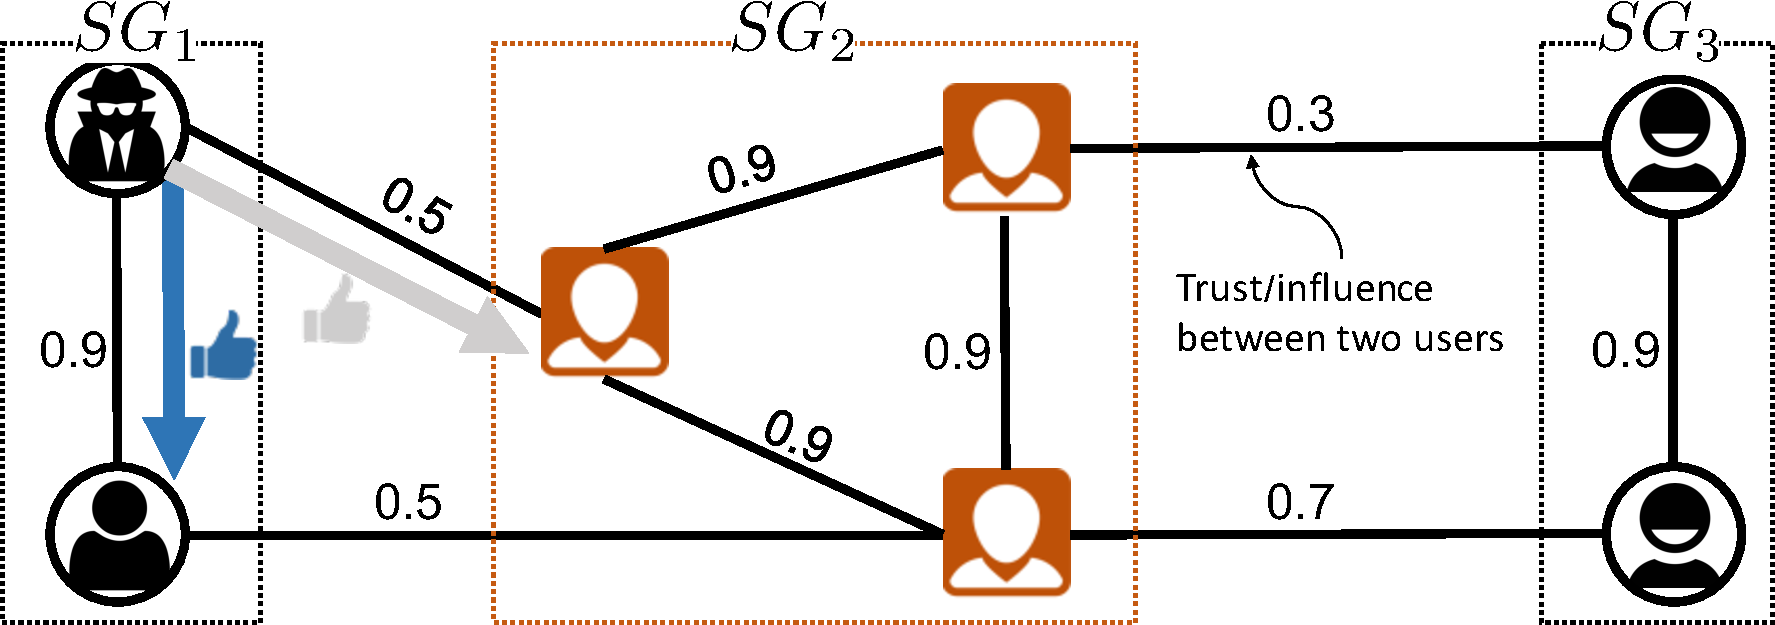
\includegraphics[height=2.3cm] {figure/motivationExampleWideWithApplication.pdf}
    \caption{ An Motivation Example}
    \vspace{-10pt}
    \label{fig:motivationExample}
\end{figure}

% \begin{figure}[t]
%     \subfigure[Social Trust Network]{\label{fig:socialNetwork}
%       \begin{minipage}[l]{0.40\columnwidth}
%         \centering
%         \includegraphics[height=2.3cm]{ill/SocialNetwork.pdf}
%       \end{minipage}
%       }
%     \subfigure[B2B Network]{\label{fig:b2bNetwork}
%       \begin{minipage}[l]{0.40\columnwidth}
%         \centering
%         \includegraphics[height=2.3cm]{ill/B2BNetwork.pdf}
%       \end{minipage}
%       }
%     \vspace{-6pt}
%     \caption{Real uncertain graphs with privacy concerns.}
%     \vspace{-10pt}
%     \label{fig:motivation}
% \end{figure} 


The rest of the paper is organized as follows. In Section~\ref{sec:relatedWork}, we summarize related works, point out the limitation of existing methods, and clarify our distinct privacy goal. In Section~\ref{sec:notation} we formulate the uncertain graph-anonymization problem. Sections~\ref{sec:soa}--\ref{sec:method} present our anonymization approach for privacy-preserving uncertain graph sharing.  In Section~\ref{sec:ex} we apply our method to several real-world uncertain graphs and demonstrate its performance, practical utility, and efficiency. 
\section{Related Work}
\label{sec:relatedWork}
A significant amount of prior work has been done on protecting the privacy of network datasets.
The comprehensive survey is out of the scope of this paper. 
Here, we briefly summarize related work and clarify our privacy goal. 

\textbf{Syntactic Privacy.}~~
Early works on privacy-preserving network releasing focus on developing anonymization techniques.
Many of them modify the graph structure in subtle ways that guarantee privacy but keep much of graph structure for release. 
The released graph is available for all the analysis tasks. 
These approaches usually provide privacy protection against specific de-anonymization attacks. 
Most of them employ syntactic privacy models derived from $k$-anonymity~\cite{Sweeney:2002:KAM:774544.774552} which requires creating $k$ same entities ({\eg} neighborhoods, degree nodes) to blend victims. 

Related anonymization methods can be classified into four main categories: (1) Clustering-based generalization~\cite{Hay_Anonymizing_2007,Bhagat_Class_2009,hay2010resisting}; (2)~{\em Edge modification}~\cite{Liu_Towards_2008, Zhou_Preserving_2008, Zou:2009, Wang2011, Wu_k_2010, Skarkala_Privacy_2012}; 
(3)~{\em Edge randomization}~\cite{Liu_Privacy_2009,Ying_Randomizing_2008, Ninggal_Utility_2015};
and~(4)~{\em Uncertainty semantic-based modifications} which add uncertainty to some edges and thus converting the deterministic graph to an uncertain version for anonymity~\cite{Boldi_Injecting_2012, Nguyen_Anonymizing_2015}. 

In the first category, Hay {\etal}~\cite{Hay_Anonymizing_2007} proposed to generalize a network by clustering nodes and only publish the hyper-graph ($\#$ of nodes in each partition with $\#$ of edges within and across partitions). Campan {\etal}~\cite{Campan2008} studied the attributed graph case with a similar solution. 
Cohen {\etal}~\cite{Cohen2013} presented a sequential clustering algorithm with better utility preserving. While, Cormode{\etal} \cite{Bhagat_Class_2009} payed attention to attributed-based matching attack. To this end, their method marks the mapping by clustering the nodes and corresponding real-world entities into groups. 

In the second category, Liu {\etal}~\cite{Liu_Towards_2008} focused on resisting degree-based entity re-identification attacks. They propose to add and delete edges to pursue $k$-degree anonymity. Zhou {\etal}~\cite{Zhou_Preserving_2008} consider stronger re-identification attack based on radius-one sub-graph. Zhou~{\etal}~\cite{Zou:2009} assume that the adversary knows the compute graph. Their algorithms use edge addition and deletion to make graph $k$-Automorphism.  

In the third category, Hay {\etal} \cite{Liu_Privacy_2009} study the use of random perturbation for identity obfuscation. They consider the basic degree-based re-identification of nodes. Besides, they propose to quantify the level of anonymity that is provided for the given node $v$ in the real network by the perturbed graph as the inverse of the maximum of the belief probability $Pr(v|u)$. Ying {\etal} \cite{Ying_Randomizing_2008} compare random perturbation methods to the method of $k-$degree anonymity. Their experiments show the deterministic edge modification methods for $k$-degree anonymity preserves the graph structure better than random perturbation methods.

The uncertainty semantic-based approaches are known as the state-of-art ones because of their excellent privacy-utility trade-off, brought by the fine-grained perturbation leveraging the uncertain semantics. 
% add two-sentences about the works 
Our method belongs to the fourth category while in the wider context. 

 
\textbf{Differential Privacy.}~~
The dependence of adversary knowledge makes graph anonymization methods are vulnerable to attackers with strong background knowledge than assumed. Such fact has simulated the use of differential privacy for more rigorous privacy guarantees. 
The recent research on applying differential privacy to graph data roughly falls into two directions. The first direction aims to release specific differentially private mining results, such as degree distributions, sub-graph counts, and frequent graph patterns~\cite{Xiao_Differentially_2014, Day:2016}. These methods only publish query result. However, there are many situations in which answering statistical queries simply does not achieve the purpose of sharing the graph.  
The second direction aims to share the meaningful graph. Most research in this direction~\cite{Sala_Sharing_2011,Proserpio_2012} projects an input graph to dK-series and ensures differential privacy on dK-series statistics. Later, private statistics are then either fed into generators or MCMC process to generate a fit synthetic graphs. However, current techniques are still inadequate to provide desirable data utility for many graph mining tasks. Wang {\etal}~\cite{Wang_2013} propose to project a graph to the spectral domain and inject noise into the eigenvalues and eigen vector. This approach achieved significant improvement in efficiency, which, is still not able to obtain useful data utility. Xiao {\etal}~\cite{Xiao_Differentially_2014} present a solution based on structural inference over the hierarchical random graph model. This approach achieved the reasonable utility over real-life graph datasets. 

As ever discussed, the state-of-art of graph privacy research has been limited to publishing data or analysis result of deterministic graphs. 
The uncertain scenario is unexplored. 
\subsection{Our Privacy Goal}
In this paper, we try to move this line of research one step forward, from the deterministic context to a broader probabilistic context.
This study focuses on generating a synthetic graph data from a real, probabilistic one under syntactic privacy guarantees. Such a synthetic graph enables scientist to draw meaningful insight while protecting the participants involved and the data collectors against risks of privacy violation. 

Another critical component is the choice of privacy notation. 
The concept of different privacy (DP) was proposed as a strong privacy measure such that sensitive information of individuals is kept private in data analysis and publishing process~\cite{Sala_Sharing_2011,Xiao_Differentially_2014}.
Immune to various privacy attacks, DP and its off-springs offers a guarantee bound $\epsilon$ on the loss of privacy due to the data release. 
While the data collector, such as e U.S. Census Bureau, has encountered many challenges in deploying differential privacy. These challenges includes, but not limited to, the difficulty in setting the value of the privacy-loss parameter, $\epsilon$ (epsilon), the lack of release mechanisms that align with the needs of data users, and the expectation on the part of data users that they will have access to micro-data~\cite{Simson:2018}. 
Recall that the trade-off between between statistical
accuracy and privacy loss is at the heart of privacy protection. 
However, Differential privacy lacks a well-developed
theory for measuring the relative impact of added noise on the utility of different data applications, tuning equity trade-offs, and presenting the impact of such decisions. 

In contrast, the notion of syntactic privacy can be defined and understood based on the data schema. And, its parameters have a clear privacy meaning that can be understood independent of the actual data. Moreover, they have a clear relationship to the privacy regulation of individual identifiability (e.g., General Data Protection Regulation).
Meanwhile, the specific utility measure can be incorporated into the privacy mechanism so that the usefulness is higher for the same privacy loss budget, allowing the overall privacy-loss budget to be better deployed.
Hence, we focus on sharing uncertain graphs with syntactic anonymity. 
\section{Problem Formulation}
\label{sec:notation}

% In this section, we provide background on uncertain graphs, privacy attack and justify our choice of utility loss metric. 
% On this basis, we present our formulation of the uncertain graph anonymization problem. 
In this section, we present background on uncertain graphs, show probabilistic privacy attacks, and formulate the privacy notion for releasing privacy-preserving uncertain graphs. We also justify our choice of utility loss metric. Finally, we present our formulation of the uncertain graph anonymization problem. 

\subsection{Uncertain Graph}
Following the mainstream literature~\cite{Potamias_K_2010,Zhao_Detecting_2014,Colbourn_Colbourn_1987}, an uncertain graph is defined over a set of nodes V, a set of edges E between nodes of V, and a probability function $\mathit{p}: E \longrightarrow 0,1 $

An uncertain graph $\mathcal{G}$ essentially represents a probability distribution over all of the certain graphs $G$ in the forms of which the uncertain graph may actually exist. 
The probability of observing any possible world $G_i=(V,E_{G_i})$ is    
\begin{equation*}
    Pr[G_i]=\prod_{e \in E_{G_i}} {\mathit{p}(e)} \prod_{e \in E \setminus E_{G_i}} 1-\mathit{p}(e)
\end{equation*}

\subsection{Probabilistic Privacy Attack}
\label{sec:AMPC}
Apparently, simply removing the identities of the nodes before publishing the uncertain graph does not guarantee privacy.  
The structure of the uncertain graph itself, and in its basic form the degree of the nodes, can be revealing the identities of individuals. 
In practice, the adversary may have access to external information about the entities in the graphs by malicious actions. 
\begin{figure}[!htb]
    \vspace{-2pt}
    \subfigure[Social Trust Network]{\label{fig:socialNetwork}
      \begin{minipage}[l]{0.46\columnwidth}
        \centering
        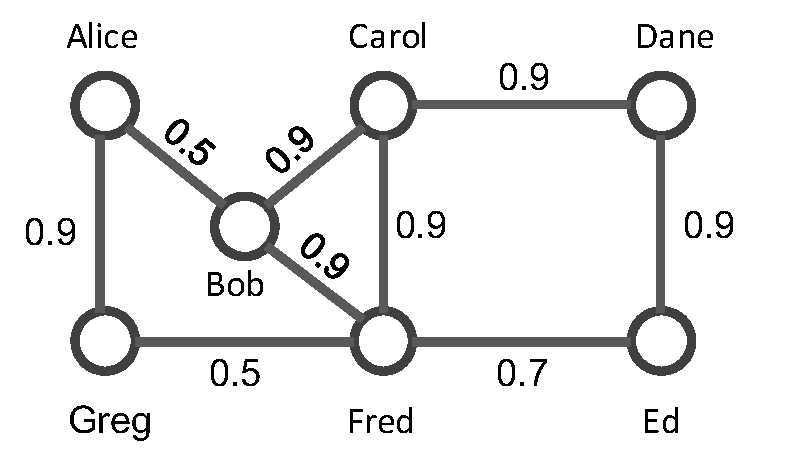
\includegraphics[height=2.7cm]{figure/example_source.pdf}
      \end{minipage}
      }
    \subfigure[The naive anonymization]{\label{fig:b2bNetwork}
      \begin{minipage}[l]{0.46\columnwidth}
        \centering
        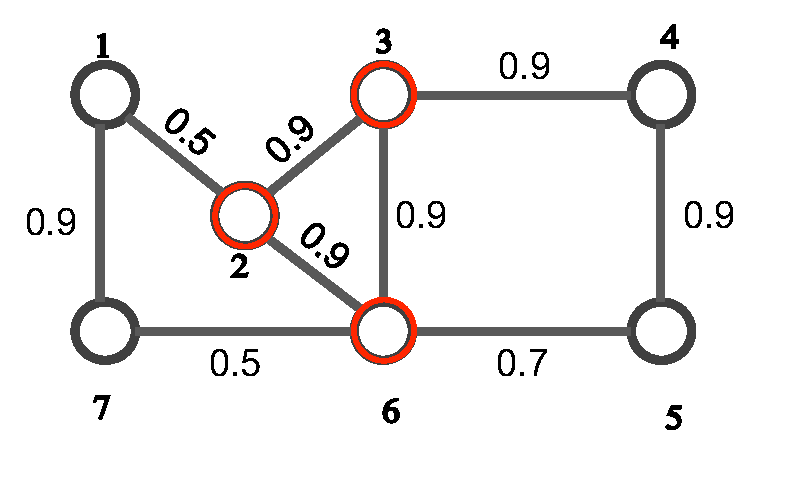
\includegraphics[height=2.7cm]{figure/example_output.pdf}
      \end{minipage}
      }
    \vspace{-4pt}
    \caption{The structural re-identification issue.}
    \label{fig:privacyAttack}
\end{figure} 
\textbf{Example.} For the uncertain graph in Figure~\ref{fig:privacyAttack}, the adversary might know that ``\emph{Fred has \textbf{three or more} trust neighbors}''. Such information allows the adversary to narrow down the set of candidates in the sanitized graphs.  The statement partially re-identify Fred as $\lbrace 2,3,6 \rbrace$ with different \textbf{probabilities} respectively. 
Different to the deterministic scenario, such posterior probabilities significantly vary over candidate nodes $\lbrace 2,3,6 \rbrace$ where $P(\text{Fred}|2) \ll P(\text{Fred}|6) \ll P(\text{Fred}|2)$ as $P(\text{Fred}|2)=0.5*0.9*0.9=0.405$ and $P(\text{Freq}|2)=0.9*0.9*0.9=0.729$ and $P(\text{Freq}|6)=0.468$. 


As ever illustrated, nodes in uncertain graphs are vulnerable to the re-identification risk. Such Entity Re-identification (ER) can lead to additional disclosures. In this work, we focus on the ER attack as it is one of the most serious privacy problems. 
\subsection{Privacy Notion}
\label{sec:privacyNotion}
In this work, we adopt $(k,\epsilon)$-obf, a variant of the well-known $k-$anonymity as the privacy notion for sharing uncertain graphs. 
It was proposed by Boldi {\etal} in ~\cite{Boldi_Injecting_2012}, where $k \ge 1$ is a desired level of obfuscation and $\epsilon \ge 0$ is a tolerance parameter. 

\textsc{Obfuscation Parameter}~~
Similar to $k$-candidate anonymity, 
$k-$obf requires blending every entity with other fuzzy matching entities. 
While, $k$-anonymity requires that each entity is identical with at least k-1 other entities. 
Bonchi{\etal}~\cite{Bonchi_Identity_2014} observed that $k$-anonymity does not measure the amount of uncertainty correctly that the adversary has regarding the correct identification of the target individual. 

$k$-obf generalizes the candidate anonymity concept to the probabilistic scenario by the use of entropy. 
For a given node $v$ in the real network, it quantifies the level of obfuscation that is provided for $v$ by the perturbed graphs as the entropy of $\lbrace Pr(v|u) : u \in V_{\hat{G}}  \rbrace$, where $Pr(v|u)$ stands for the posterior belief probability that $u$ is the image of the target node $v$. 

% It lower bounds the entropy of the distribution by $\log_{2}k$.
Though it is initially used to measure the anonymity provided by an uncertain graph to the deterministic graph, the stochastic nature makes it a good fit in the uncertain scenario. 

\textsc{Tolerance parameter}~~As for the tolerance parameter $\epsilon$, it serves for the following purpose. There might be extreme unique nodes, e.g., Trump in a Twitter network, whose obfuscation is almost impossible. Thus, Boldi {\etal} introduce a tolerance parameter $\epsilon$, which allows skipping up to $\epsilon * |V|$ nodes and makes the privacy notion more practical. 
% The formal definition is,
% \theoremstyle{definition}
% \begin{definition}
%     \textbf{\boldmath{$(k,\epsilon)$}-obf \cite{Boldi_Injecting_2012}}
%     Let $P$ be a vertex property (i.e., vertex degree in our work), $k \geq 1$ be a desired level of anonymity, and $\epsilon >0 $ be a tolerance parameter. 
%     An sanitized uncertain graph $\tilde{\mathcal{G}}$ is said to $k$-obfuscate a given vertex $v \in \mathcal{G}$ w.r.t $P$ if the entropy $H()$ of the distribution $Y_{P(v)}$ over the nodes 
%     of $\tilde{\mathcal{G}}$ is greater than or equals to $\log_{2}{k}$:
%     \begin{equation*}
%         H(Y_{P(v)}) \geq \log_{2}{k}.
%     \label{obfCon}
%     \end{equation*}
% The uncertain graph $\tilde{\mathcal{G}}$
% is $(k,\epsilon)$-obf w.r.t property $P$ 
% if it $k$-obfuscates at least $(1-\epsilon)|V|$ nodes in $\mathcal{G}$. 
% \label{def:obf}
% \end{definition} 
\subsection{Reliability-oriented Utility Metric}
% In this work, we use reachability discrepancy as the utility-loss metric for utility safeguard.
\begin{figure}[!htb]
  \centering
  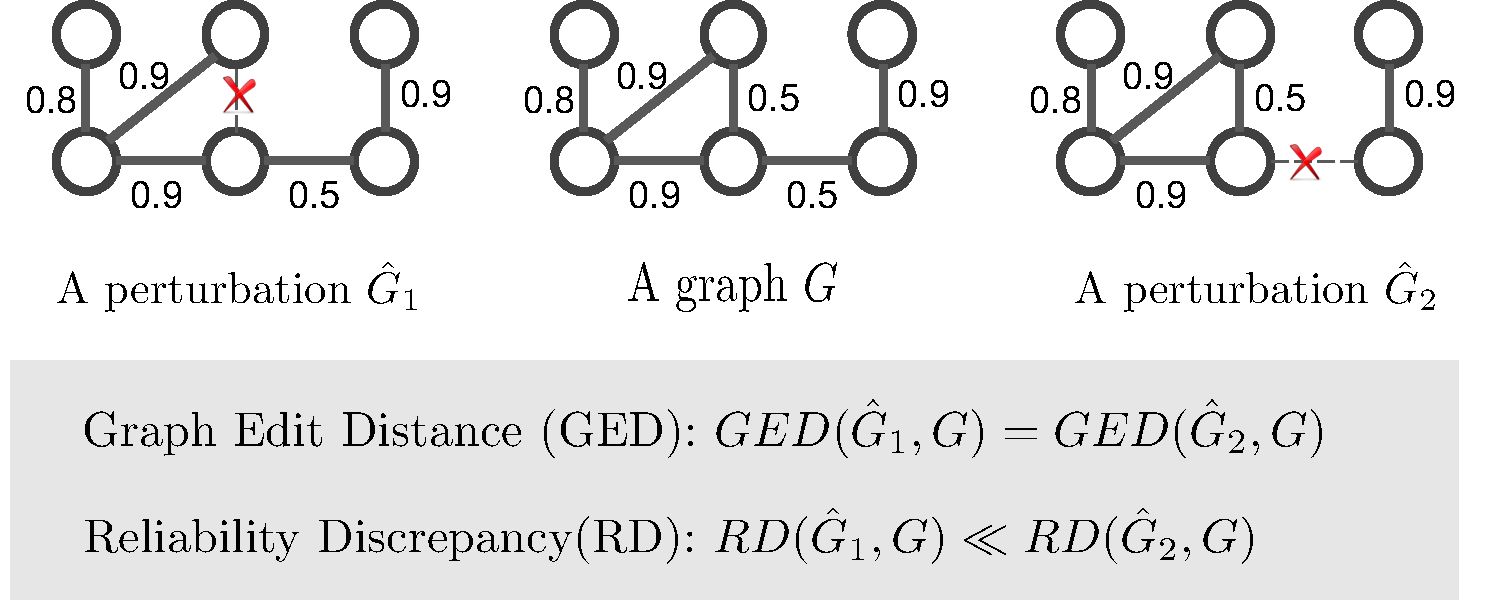
\includegraphics[height=3.2cm]{figure/utilityLoss.pdf}
  \vspace{-10pt}
  \caption{Comparison of utility loss metrics.}
  \label{fig:utility_loss}
\end{figure} 
% In the context of deterministic graphs, connectivity discrepancy is widely used to measure the structural distortion for the following reasons. 
% First, the connectivity model is known to yield a better graph representation than the degree sequence model.
% What's more, connectivity plays a vital role in various graph mining tasks such as nearest neighbor locating, decomposition and graph clustering. 
% While, the concept of reliability generalizes the connectivity concept in the uncertain scenario. 
% It captures the probability that two given nodes are reachable over all possible worlds, as shown in Def~\ref{d:reliability}. 
For uncertain graphs, reachability is not a simple Yes/No question, but instead, a probabilistic one. 
\begin{definition}
    \textbf{Reliability~\cite{Colbourn_Colbourn_1987}}~In uncertain graph $\mathcal{G}$, reachability from node $u$ to node $v$ is expressed as the overall probability of those possible graphs of G in which $u$ can reach $v$. 
        \begin{equation*}
                R_{u,v}(\mathcal{G})= \sum_{G \in W(\mathcal{G})} \mathcal{I}_{G}(u,v) ~ Pr[G] 
        \end{equation*}
    where Pr[G] is the probability of observing $G$ as one possible world of G, and $\mathcal{I}_{G}(u,v)$ is 1 iff $u$ and $v$ are contained in a connected component in $G$, and 0 otherwise.   
    \label{d:reliability}
\end{definition}

\theoremstyle{definition}
\begin{definition}
    \textbf{Reliability Discrepancy (RD)}
    The reliability difference between a sanitized output $\tilde{\mathcal{G}}$ and the original input $\mathcal{G}$, 
    denoted as $\Delta(\tilde{\mathcal{G}})$, 
    is defined as the sum of the two-terminal reliability discrepancy over all node pairs $(u,v) \in V_\mathcal{G}$.
    \begin{equation*}
        \Delta(\tilde{\mathcal{G}})=\sum_{(u,v) \in V_\mathcal{G} }|R_{u,v}(\mathcal{G})-R_{u,v}(\tilde{\mathcal{G}})|
    \end{equation*}
    \label{d:RD}
\end{definition}

\subsection{Problem Statement} 
% \vspace{-5pt}
\begin{problem}
     Given an uncertain graph $\mathcal{G}$ and desired anonymization parameters $k$ and $\epsilon$, 
     the objective is to find a  $(k,\epsilon)$-obf uncertain graph $\tilde{\mathcal{G}}$
     with the minimal utility loss,
     \begin{equation*}
             \begin{aligned}
                 & \argmin_{\tilde{
                \mathcal{G}}} & & \Delta(\tilde{\mathcal{G}}) \\
                &  \text{Subject to} & &\tilde{\mathcal{G}} \text{~is~} (k,\epsilon)-obf
            \end{aligned}
     \end{equation*}
     \label{prob:unobf}
\end{problem}
% add one paragraph to ....
\section{The State-of-Art Approach}
\label{sec:soa}
Before presenting our solution {\methodName}, we first describe the state-of-art deterministic graph anonymization approach ({\soaName})~\cite{Boldi_Injecting_2012}.
The purpose of describing it is to separate the basic framework with the contribution of {\methodName}. 
They differ in the search strategy of sanitized candidates.  

\subsection{Overview}~~
The {\soaName} method obfuscates the (deterministic) graph data by adding or removing edges \emph{partially}. 
For each edge $e$, it assigns a probabilistic deviation $r_{e} \in [0,1]$, where $r_{e} \leftarrow R(\sigma)$. 
In particular, the uncertainty injecting scheme proceeds as follows:
\begin{equation}
    p(e) =
    \begin{cases}
         1-r_{e}  & e \in E \\
         r_{e}    & otherwise 
    \end{cases}
    \label{eq:inject}
\end{equation}
Generally, it transfers edge existence from existing edges to non-existing ones for identification obfuscation.   

\begin{figure}[htb]
  \centering
        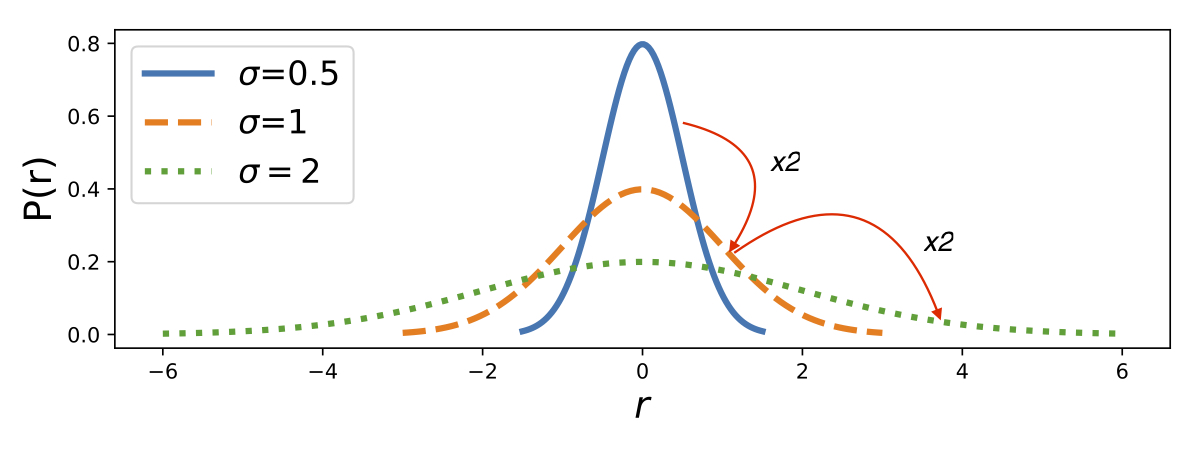
\includegraphics[width=0.8\linewidth]{figure/std_2.jpg}
  \vspace{-5pt}
  \caption{Illustration of the obfuscation effect brought by larger values of standard deviation $\sigma$.}
  \vspace{-5pt}
  \label{fig:std}
\end{figure} 

For the high utility of the obfuscated graph, smaller values of the parameter $r_{e}$ should be favored.  
The most widely known member of generating distribution $R({\sigma})$ is the truncated normal distribution with mean 0 and variance $\sigma^2$. 
In principle, $R$ could be any distribution.
As the standard deviation $\sigma$ decreases, a greater mass of $R_{\sigma}$ will concentrate near $r_{e}=0$.  
As illustrated in Figure~\ref{fig:std}, smaller values of $\sigma$ generally contributes towards better utility preserving, while at the same time they provide lower level of obfuscation. 
Larger values of $\sigma$ have the opposite effect.
Then, the amount of injected noise and consequent structural distortion will be smaller. 
Aiming at the high utility, {\soaName} aims at injecting the minimal amount of uncertainty need to achieve the necessary obfuscation. 
As outlined in Algo~\ref{alg:obf}, it computes the minimal amount of uncertainty via a binary search on the $\sigma$ value. 
\begin{algorithm}
    \begin{algorithmic}[1]
    	\item[] {\textbf{Input:}~Graph $\mathcal{G}$, obfuscation level $k$, tolerance parameter $\epsilon$}
        \item[] {\textbf{Output:}~The result $\mathcal{G}_{obf}$}
     	\STATE {$\sigma_{l} \leftarrow 0$; $\sigma_{u} \leftarrow 1$} \\
        \REPEAT
        \STATE{$\langle \hat{\epsilon}, \hat{\mathcal{G}} \rangle$ $\leftarrow$ \textbf{genObf}(-,$\sigma_{u}$)} \\
        \STATE{{\bf if} $\hat{\epsilon}=1$ (fail) {\bf then} $\sigma_{l} \leftarrow \sigma_{u}$; $\sigma_{u} \leftarrow 2\sigma_{u}$}
        \UNTIL{$\hat{\epsilon} \neq 1 $} \\
        \REPEAT
        	\STATE {$\sigma_{mid} \leftarrow (\sigma_{u}+\sigma_{l})/2$}
            \STATE{$\langle \hat{\epsilon}, \hat{\mathcal{G}} \rangle$ $\leftarrow$ \textbf{genObf}(-,$\sigma_{mid}$)}
            \STATE {{\bf if} $\hat{\epsilon} =1$~{\bf then}~$\sigma_{l} \leftarrow \sigma_{mid}$}\\
            \STATE {{\bf else} $\sigma_{u} \leftarrow \sigma_{mid}$;~~{$\mathcal{G}}_{obf} \leftarrow \hat{\mathcal{G}}$}
        \UNTIL{$\sigma_{u}-\sigma_{l}$ is enough small}
        % \COMMENT{\textcolor{blue}{\scriptsize Binary search for better obfuscation}}
        \STATE {return $\mathcal{G}_{obf}$}
    	\caption{The obfuscation algorithm}
	 \label{alg:obf}
    \end{algorithmic}
\end{algorithm}


The function genObf, which aims at generating {\keobf} instances using a given standard deviation parameter $\sigma$, determines the search flow. It either returns the generated sanitized instance or the failure signal.
The search starts with an initial guess of an upper bound $\sigma_{u}$, which is iteratively doubled until a {\keobf} instance is found. Then, the binary search is performed over the range $[0,\sigma_{u}]$. The binary search terminates until the search interval is sufficiently short. The algorithm outputs the best found sanitized output  (the last one that was successfully generated; the one with the smallest $\sigma$).

\subsection{GenObf Function}
% It is difficult to find {\keobf} sanitized solutions using a given parameter $\sigma$ over the intractable search space. 
The genObf function separates the search process into running two independent modules: (1) uncertain noise generative models and (2) privacy tests. 
The first constructs a utility-preserving noise generative model. 
Meanwhile, the privacy test aims to safeguard the privacy of generated obfuscation. 
Overall, it leverages random search to alleviate the combinational intractability.  
Particularly, multiple randomized attempts are performed. 
Every obfuscated output is subject to this privacy test. 
Iff all the attempts fail, {\genobf} returns failure sign. Otherwise, it returns the found {\keobf} instance.

Each construction attempt begins with selecting a subset of edges subject to alteration. 
Then, it assigns the deviation among selected edges and injects uncertainty. 
While, the randomization process heavily relies on the heuristic.  
In particular, {\soaName} suggests calibrating the perturbation applied to an edge $e$ according to the ``uniqueness" of the two nodes $u$ and $v$. 
In brief, if both $u$ and $v$ are common nodes {\wrt} the property, then $r_{e}$ should be very small; 
on the other hand, if $u$ and $v$ are outliers, then $r_{e}$ should be higher. 
Meanwhile, edges need to be sampled with the higher probability if they are adjacent to outliers. 

\subsection{Limitations} 
The {\soaName} method provides the desired level of privacy guarantee with the small change in the graph, thus maintaining high utility.
However, this method has two critical weaknesses in the probabilistic context:
(1) The design heavily tailored towards the deterministic scenario {\eg} it assumes the existence of edges is binary (0,1). Thus, it fails to handle uncertain graphs where the existence of edges is probabilistic. 
All the operators, including edge selection and alteration, need to be integrated with possible world semantics carefully.
(2) Its scheme does not consider the structural relevance of edges in critical edge selection/alteration steps, which leads to unnecessary structural distortion.
We are left asking the following questions, \emph{how to generalize existing methods to the probabilistic context?} and \emph{how to get a better trade-off between privacy and utility in the probabilistic context?} 
\section{Privacy Via {\capMethodName}}
\label{sec:method}
In this section we describe our algorithm, {\methodName}, which injects uncertainty to the given uncertain graph so that it becomes {\keobf} while preserving as much the stochastic nature as possible. 
A key feature of our method is to seamlessly integrate edge uncertainty and possible world semantics into the core of anonymization operators.
% 

\subsection{Heuristic for Edge Perturbation}
in graph anonymization, selecting edges which subject to modification, is often considered as the most central operation,as well as the most complex one. 
It needs to balances privacy gain and structural distortion. 
For the graph, it often needs to consider of the exponential number of edge combinations. 
Recently, the most popular paradigm for solving such problems has been using a class of heuristics. 
Successes of this approach include
(1) anonymity-aware ones that suggest injecting more considerable noise to unique nodes~\cite{Ying2009,Boldi_Injecting_2012,Hay_Anonymizing_2007} 
(2) utility-aware ones that avoid distortion over ``bridge" edges whose deletion/addition would significantly impact the graph structure~\cite{Wang2011,Ninggal_Utility_2015}. 
Clearly, the judicious edge selection must involve two types of heuristics which complement each other. While, they have not been explored yet in the probabilistic context.

In this work, we first generalize the calibration of ``uniqueness" with the marriage of KL-divergence function. 
Second, from the information-theoretic perspective, we propose a generalized version of edge relevance. 
Beside, we describe an efficient algorithm for probabilistic edge relevance evaluation.
Then, we show how to use multi-heuristics to boost anonymization efficiently and straightforwardly.

\textbf{Generalized Uniqueness}~~
The uniqueness criterion quantifies how unique a given node is among all the nodes in the graph {\wrt} a specific property $P$. 
More specifically, the uniqueness of a node $v$ is defined as the harmonic mean of property distances against all other nodes {\wrt} a specific property. 
However, the conventional method merely formulates node properties as discrete values and relies on the geometric distance function to measure their distances.  
It fails to handle uncertain graphs where the property values are probabilistic.

\begin{figure}[!htb]
  \centering
        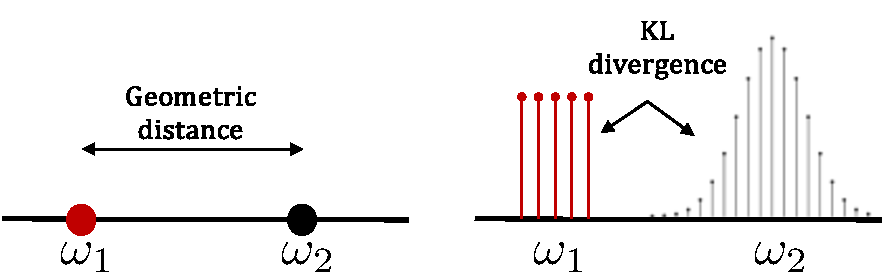
\includegraphics[width=\linewidth]{figure/unique.pdf}
  \caption{The generalization of uniqueness.}
\end{figure}

We extend the preliminary version to handle the probabilistic case. 
We first systematically model uncertain property values in both continuous and discrete domains as continuous and discrete random variables, respectively.
Then, we consider the use of probability distributions, which are essential characteristics of uncertain property values, in the measuring similarity between uncertain property values. 
In this work, we use the well known Kullback-Leibler divergence to measure the distance between random variables with parameterized distributions. 

\begin{definition}
    \textbf{Uniqueness Score}
    Let $P$ be a property on the set of nodes $V$ of the input graph ,  
    let $d$ be the KL divergence function, 
    and let $\theta >0$  be a parameter. 
    Then the $\theta$-commonness of the property values $\omega$
    is $C_{\theta}(\omega)$ amounts to a weighted average over all other property values $\omega'$.    
     while the corresponding uniqueness is $U_{\theta}:= \frac{1}{C_{\theta}(\omega)}$. 
    \vspace{-5pt}
\end{definition} 
In the above definition, the weights decays exponentially as a function of the KL divergence among property values, 
and the parameter $\theta$ determines the decay rate. 
\begin{equation*}
  C_{\theta}(\omega) = \sum_{u \in V} \Phi_{\theta}(KL(\omega, P(v)))
\end{equation*}
In this work, we set $\theta=\sigma$ as the injected noise blurs the meta-distribution of property values. 
 
\textbf{Generalized Edge Relevance}~~
Alteration over a single edge would produce local structural change and send ripples through the rest of the graph. 
Even with the same amount of deviation, the incurred structural distortion varies on the topological role of the altered edge. 
Targets at the high utility, we should penalize edge modifications according to the incurred structural distortion.  
It naturally raises the need of measuring the relevance of edges in the probabilistic context. 

There are many potential ways to measure it. 
Importantly, the metric should be able to capture key properties of uncertain graphs.
Inspired by the importance of reliability, we measure the edge relevance of a given edge $e$ as the amount of structural distortion, measured by reliability discrepancy, caused by the unit noise subjects to the edge $e$, as follow. 
\begin{equation*}
  \begin{split}
    \mathcal{ERR}({e}) &= \frac{\Delta(\mathcal{G}+r_{e})}{|r_{e}|}  \\
                       &= \frac{\sum_{u,v} |R_{u,v}(\mathcal{G}+r_{e}) -R_{u,v}(\mathcal{G})|} {|r_{e}|}
  \end{split}
\end{equation*}

In the conventional case (deterministic graphs with edge addition and deletion $|r_{e}|=1$), it amounts to the connectivity distortion, measured by the deviation of \# of connected node pairs.  
In probabilistic graphs, $\mathcal{ERR}$ is used to generalize this concept by quantifying the stochastic impact of partial edge addition/deletion ($r_{e}$ lies in the contentious range) over the connectivity of all the possible worlds.
% It allows the estimation of structural distortion when $r_{e}$ lies in the contentious range. 
\begin{observation}
  Let $\mathcal{G}_{e}$, $\mathcal{G}_{\bar{e}}$ 
  denote two uncertain graphs that are identical to $\mathcal{G}$ with $p(e)=1$ and $p(e)=0$ respectively. 
  The reliability relevance of an edge $e$ is a constant and equivalent to 
  the following function. 
  \begin{equation}
    \mathcal{ERR}(e) = \sum_{u,v} R_{u,v}(\mathcal{G}_{e}) \big- \sum_{u,v} R_{u,v}(\mathcal{G}_{\bar{e}})
    \label{eq:err}
  \end{equation}
  Observe that, the edge relevance only depends on it topological location. 
  It amounts to the difference of the number of connected pairs between two neighbor uncertain graphs. 
\end{observation}

\textbf{Proof Sketch.}~~
According to the possible world semantics and factorization rule, we can see that   
\begin{equation*}
  R_{u,v} (\mathcal{G}) = p(e) \cdot R_{u,v}(\mathcal{G}_{e}) ~+~ \big[ 1-p(e) \big] \cdot R_{u,v} (\mathcal{G}_{\bar{e}})
\end{equation*}
Note that, the two-terminal reliability $R_{u,v}$ in $\mathcal{G}_{e}$ and $\mathcal{G}_{\bar{e}}$ are constants. 
Therefore, two-terminal reliability discrepancy introduced by the single deviation $r_{e}$ over the uncertain graph $\mathcal{G}$ is equivalent to 
\begin{equation*}
  \begin{split}
    \Delta_{u,v} (\mathcal{G}+r_{e}) ~&= r_{e} \cdot R_{u,v}(\mathcal{G}_{e}) - r_{e} \cdot R_{u,v} (\mathcal{G}_{\bar{e}})\\
    &= r_{e} \cdot ~\big[  R_{u,v}(\mathcal{G}_{e}) - R_{u,v} (\mathcal{G}_{\bar{e}})  \big]
  \end{split}
\end{equation*}
After aggregation and eliminating the factor $r_{e}$, we can see that the reliability relevance of an edge $e$ is equivalent to Equation~\ref{eq:err}. $\square$

Equation~\ref{eq:err} reminds us the basic concept of cut-edge. 
% What is the relationship between Equation~\ref{eq:err} and the conventional cut-edge definition? 
In a deterministic graph, a cut-edge is an edge of a graph whose deletion increase its number of connected components. 
We can see that the cut-edge is a binary version of $\mathcal{E}RR$.  
While $\mathcal{E}RR$ is a continuous function regarding the edge deviation $r_{e}$ and reliability discrepancy. 
$\mathcal{E}RR$ is not only relevant to connectivity discrepancy but also consider its scale.  

\textbf{Re-visiting the Computation Challenge}~~
\begin{figure}
    \subfigure[Iterative Evaluation]{\label{fig:itERR}
      \begin{minipage}[l]{0.46\columnwidth}
        \centering
        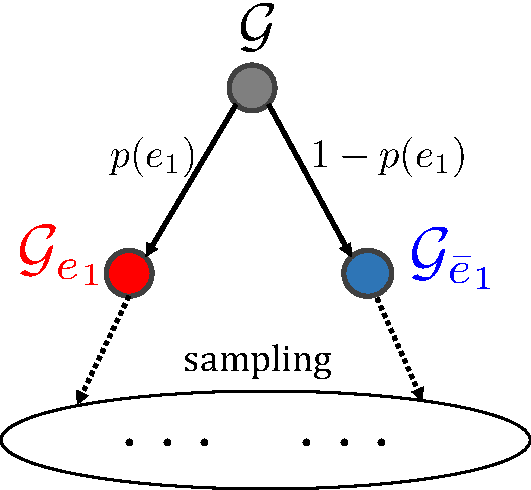
\includegraphics[height=2.7cm]{figure/iterativeERR.pdf}
      \end{minipage}
      }
    \subfigure[Memorized Evaluation]{\label{fig:groupERR}
      \begin{minipage}[l]{0.46\columnwidth}
        \centering
        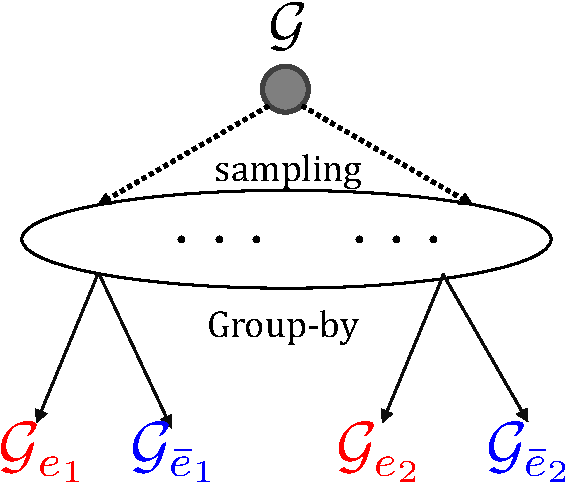
\includegraphics[height=2.7cm]{figure/groupERR.pdf}
      \end{minipage}
      }
    \vspace{-10pt}
    \caption{Sampling-based reliability detection}
    \vspace{-5pt}
    \label{fig:computationERR}
\end{figure} 
% At the first glance, the evaluation of $\mathcal{E}RR(e)$ 
The remaining question is to calculate
As shown in Equation~\ref{eq:err},  
the evaluation of $\mathcal{E}RR(e)$ involves a fundamental problem concerning uncertain graphs, which we call 
the Two-Terminal Reliability detection (TTR) problem. 
Since this problem is \#P-complete, we focus on efficiently and accurately approximate TTR.
The Monte-Carlo sampling method can be used to estimate the underlying reliability of an uncertain graph. 
Namely, we create a subset of possible worlds of the given uncertain graph with the use of edge sampling probabilities. 
Then, we take the average of the number of connected node pairs in the sampled worlds as an approximation. 
 
It is not trivial to evaluate $\mathcal{E}RR$ over all the edges. 
One option is to iteratively invoke the sampling-based reliability computation over all the edges, 
as illustrated in Figure~\ref{fig:itERR}. 
It is straightforward to compute the connected components of a graph in linear time (regarding the numbers of the nodes and edges of the graph) using either breadth-first search or depth-first search.
For each edge, we need to perform the connected component detection for $N$ sampled graphs.
Thus, the overall time complexity is typically in the order of $\mathcal{O}( N |E|^{2})$.
Apparently, the iterative evaluation is inefficient when the uncertain input graph is massive.

Here, we present an efficient method with the time complexity in the order of $\mathcal{O}(N |E|)$.
As illustrated in Figure~\ref{fig:groupERR}, it memories the connected components detection result of samples. 
For evaluating the reliability relevance of one edge $e$, we group the sampled possible worlds according to the edge existence, 
then get the average value of $cc$ over each group as accurate approximation of $cc(\mathcal{G}_{e})$ and $cc(\mathcal{G}_{\bar{e}})$. 
Instead of sampling and evaluation from the scratch, we utilized the memorized results. 
The running time analysis roughly follows the analysis of the single-edge case.  
By this way, we bring the evaluation of edge reliability relevance to the realm.

\textbf{Edge Selection Boosted by Multi-heuristics}~~
To get the balance between anonymity and utility, we combined the generalized uniqueness metric $U$ and relevance $R$ metric by taking the ratio between them. 
We denote the combination as Balance Factor (BF) which is defined as follows:
\begin{equation*}
    BF(v)=\frac{U(v)}{R(v)}
\end{equation*}
For a give vertex $v$, $U(v)$ is the normalized uniqueness score of its property value among all the node in the original graph; $R(v)$ is the sum of reliability relevance of edges adjacent to the vertex. 
The higher value of BF represents the better trade-off between anonymity preserving and utility preserving. 
Our algorithm uses this heuristic to select and perturb the edge of uncertain graphs, as outlined in Algorithm 2. 




 % hybrid Heuristic
\subsection{Stochastic Uncertainty Injecting Scheme}
For each sampled edge $e$ with the distributed standard deviation $\sigma_{e}$, we select the probability deviation $r_{e}$ where $r_{e} \leftarrow R_{\sigma_{e}}$. 
Thus, the remaining question is \emph{how can we safely alter edge probability for higher anonymity?}
Given the deterministic graph, the idea of uncertainty injecting is to transfer probabilities from existing edges to potential edges, as outlined in Equation~1.
However, the uncertainty injecting scheme is unexplored in the uncertain scenario.  
\begin{figure}[!htb]
  \centering
        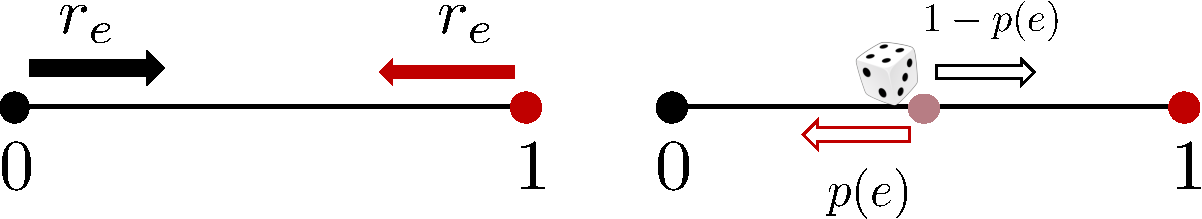
\includegraphics[width=\linewidth]{figure/uncertaintyInjecting.pdf}
    \caption{The generalized uncertainty injecting scheme.}
\end{figure}
There are many potential ways to extend the uncertain injecting scheme to the probabilistic context.   
One option is the Most-Provable-Scheme where the edge probability alteration follows the most probable policy.
\begin{equation*}
  p(e) =
  \begin{cases}
     p(e)-r_{e}    & p(e) \ge 0.5 \\
     p(e)+r_{e}    & otherwise 
  \end{cases}
  \label{eq:inject}
\end{equation*}

Another simple alternative is to consider the probability the edge exists as an indicator of the scheme. 
It performs the following uncertainty injecting scheme.
\begin{align}
  p(e)~&=~ [p(e)] \cdot (1-r_{e})+ [1-p(e)] \cdot r_{e} \\
      ~&=~ p(e) + \big[ 1- 2 p(e) \big] \cdot r_{e}
  \label{eq:ui}
\end{align}
It has already been used as the uncertainty injecting scheme in our previous work~\cite{Xiao:2018}; 
The flexible value of the edge probability is limited to the range between $p(e)$ and $1-p(e)$.
Intuitively, it requires maximizing degree entropy/variance. 

However, its connection to the core anonymity objective and the mathematical foundation are unclear. 
In this work, we show the stochastic uncertainty injecting scheme can maximize the related objective function of anonymity.  

\textbf{The relaxed version of anonymity}~~
To simplify the discussion, let us consider the primary case $k$-obf which low bounds the entropy of posterior-probability distribution over all the nodes.  
It imposes a set of hard constraints on the output solution. 
To make it formal, let us define the set of feasible solutions satisfying all the constraints as:
\begin{equation*}
  \{\pg~~s.t.~~ \forall v ~\mathrm{E}(v) \ge  \log k \}. 
\end{equation*}
$k-$obf can be expressed as joint satisfaction of a set of constraints 
since the uncertain graph is said to be $k$-obf iff it $k-$obfuscates all the nodes. 
Then, in order to sanitize graph, we could maximize the following function: 
\begin{equation*}
    \mathcal{F}_{e} = \prod_{v \in V} \mathcal{C}_{v}              
\end{equation*} 
where 
\begin{equation*}
  \mathcal{C}_{v} = 
  \begin{cases}
    1 & \mathrm{E}_{v} \ge  \log k \\ 
    0 & otherwise 
  \end{cases}
\end{equation*}

The single constraint {\Constraint} is either fully satisfied or thoroughly violated. 
The discontinuity limits the opportunity of gradient-based optimization methods.
The connection between our objective function is still unclear.  
Thus, we relax the single constraint {\Constraint} to a fuzzy relation as: 
\begin{equation*}
  \mathcal{C}_{v} = e^{\mathcal{E}_{v}-\lambda}.
\end{equation*}
Then, the satisfaction becomes a continuous and differential function {\wrt} the entropy. 
It turns out that the problem can be reduced to maximizing a much simpler function with the relaxed version of anonymity.  

\begin{observation}
  The maximization of $\mathcal{F}_{e}$ is equivalent to the maximization of the following function:
  \begin{equation*}
    \mathcal{F} =  \sum_{v\in V} E(v) - \Number E(\Omega)
  \end{equation*}
\end{observation}
Targeting at high utility, it aims at increasing the uncertainty at the vertex level $\sum_{v \in V} E(v)$. 

\textbf{Proof Sketch.}~~
Let $\Omega$ presents the domain of property values in the given graph; we can see that 
\begin{equation*}
  \mathcal{F}_{e} = \prod_{\omega \in \Omega} \underbrace{\mathcal{C}_{\omega} \ldots \mathcal{C}_{\omega}}_{s(\omega)}, 
\end{equation*}
Taking logarithm for both sides and combining the approximation, our goal is actually to maximized 
\begin{align*}
  \log \mathcal{F}_{e} &= \sum_{\omega \in \Omega} s(\omega)~\log C(\omega) \\
                       &= \sum_{\omega \in \Omega} s(\omega) \big[ E(\omega) - \lambda \big] \\
                       &= \sum_{\omega \in \Omega} s(\omega) E(\omega) ~-~ \Number \lambda 
\end{align*}
Therefore, after removing the constant $\Number\lambda$, our goal is actually to maximize 
$\sum_{\omega \in \Omega} s(\omega) E(\omega)$. 
It bridges the anonymity of the overall graph $\mathcal{F}_{e}$ 
with the component coding (the disorder) of the fuzzy matching matrix. 

To perform data coding, we have two angles, row  and column, that gain the same result of coding length $\mathcal{L}$ as:
\begin{align*}
  \mathcal{L} &= \sum_{v \in V} E(v) + \Number \log \Number                             &(row)\\
              &= \sum_{\omega \in \Omega} s(\omega) E(\omega)~+~\Number E(\Omega) &(column). 
\end{align*}
Therefore, after removing the constant $\Number \log \Number$, our goal is actually to maximize 
$\mathcal{F}_{e}$. $\square$  

\begin{observation}
  Equation~\ref{eq:ui} approximates the gradient-based exploration of the simplified objective function $F$.
\end{observation}

\textbf{Proof Sketch.}~~
Fix such node $v \in \mathcal{G}$ and let $e_{1},\ldots, e_{l}$ be $l$ edges that include $v$. 
Letting $d_{v}$ be the random variable corresponding to the degree of $v$, 
we have 
\begin{equation*}
  d_{v} ~=~ \sum_{i}^{l} p(e_{i}). 
\end{equation*}
As ever described, {\methodName} selectively modifies edges connected to unique nodes ({\ie}, nodes with high degree).
The degree of such node $v$ can be approximated by the normal distribution. (The Central Limit Theorem becomes effective already for $l\approx 30$; for unique nodes in the real uncertain graph, the approximation becomes accurate enough.) We have
\vspace{-5pt}
\begin{align*}
   d_{v}~&\sim~\mathcal{N}(u, \sigma^2); \\
   \sigma^{2}~&=~\sum_{i=1}^{l} Var(P(e_{i}))=\sum_{i=1}^{l} p(e_{i}) (1-p(e_{i}))
   \vspace{-15pt}
\end{align*}
The entropy of the random variable, $E(v)$, can then be approximated by the differential entropy of the normal distribution as ${{1}\over{2}}{\ln (2\pi\sigma^2)}+ {{1}\over{2}}$. 
The gradient of our objective function {\wrt} the edge existence  can be rewritten as
\begin{align*} 
  \nabla \mathcal{F}~&=~\nabla E_{v}~=~\nabla \ln(\sigma^2) \\
                    ~&\sim \frac{1}{\sigma^2} \nabla \sigma^{2}~\sim~\frac{1}{\sigma^2} \big [ 1-2~p(e_{i}) \big].~\square
\end{align*} % uncertainty Injecting 
\subsection{The {\methodName}-obf Algorithm}
\begin{algorithm}[!htb]
	\begin{algorithmic}[1]
    	\item[] {\textbf{Input:}~Uncertain graph $\mathcal{G}$, the desirable obfuscation level $k$, \
                tolerance parameter $\epsilon$, the standard deviation $\sigma$, $t=5$ five attempts and auto tuned size multiplier $c$.}
        \item[] {\textbf{Output:}~A pair of the sanitized output $\mathcal{G}_\text{obf}$ and $\hat{\epsilon}$.}
        \STATE {Compute the generalized uniqueness score $U$}
        \STATE {Compute the reliability relevance $R$}
        \STATE {Get $\mathcal{H}$:~$\frac{\epsilon}{2}\Number$ nodes with highest $U(v)R(v)$ score}
        \STATE {Compute and normalize balance factor $BF(v)=\frac{U(v)}{R(v)}$}
        \STATE {$\hat{\epsilon} \leftarrow 1$}
   		\FOR{$t$ times} 
         	\REPEAT  
                \STATE {$E_{C} \leftarrow E$} 
            	\STATE{randomly pick a vertex $u \in V \setminus \mathcal{H}$ according to $BF$}
            	\STATE{randomly pick a vertex $v \in V \setminus \mathcal{H}$ according to $BF$}
                \IF {$(u,v) \in E$}
                    \STATE {$E_{C} \leftarrow E_{c} \setminus \lbrace(u,v)\rbrace$ with the probability $p(e)$}
                \ELSE
                    \STATE {$E_{c} \leftarrow E_{c} \cup \lbrace(u,v)\rbrace$}
                \ENDIF
            \UNTIL{$E_{C}=c|E|$}
            \FORALL {$e \in E_{C}$} 
            	\STATE {Compute $\sigma(e)$}
                \STATE {Generate $r_{e} \leftarrow R_{\sigma(e)}$}
                \STATE {Inject uncertainty: $p(e) \leftarrow p(e) + \big[ 1- 2 p(e) \big] \cdot r_{e}$}
            \ENDFOR
            \STATE {$\epsilon_{s} \leftarrow anonymityEvaluation(\mathcal{G}_{s})$ }
            \IF {$\epsilon_{s} < \text{min}(\hat{\epsilon},\epsilon)$}
                \STATE {$\hat{\epsilon} \leftarrow \epsilon_{s}$, $\mathcal{G}_\text{obf} \leftarrow \mathcal{G}_{s}$}
            \ENDIF 
        \ENDFOR 
        \STATE {return $\langle \hat{\epsilon},  \mathcal{G}_\text{obf} \rangle$}
      	\caption{Squid-genObf}
        \label{alg:squid}
    \end{algorithmic}
\end{algorithm}

The {\methodName}-obf performs following steps to judiciously use the ``uncertainty budget" $\sigma$.

[Line 1-2]~It computes the uniqueness and relevance level for each vertex $v \in V$. 
The more unique a vertex is, the harder it is to obfuscate it. 
The more relevant a vertex is, the more significant impact the mutation brings.

[Line 3]~It first select the set $\mathcal{H}$ of $\frac{\epsilon}{2}\Number$ nodes, and exclude them from the subsequent mutation effort. Instead of excluding the nodes requires most considerable mutations (uniqueness), {\methodName}-obf also excludes the ones with significant structural relevance. 

[Line 4]~The mutation over edges is needed to obfuscate the set of nodes not in $\mathcal{H}$. 
Higher uncertainty is necessary t obfuscate  ``outliers", nodes with higher uniqueness score. 
Thus, edges need to be sampled with the higher probability if they are adjacent to unique nodes. 
Mutation over ``bridge-like" edges need to be minor to preserve data utility. 
Thus, edges with higher relevance score need to be sampled with lower probability.
We utilize two complementary heuristics, uniqueness (the anonymity-aware one) and relevance (the utility-aware one) to guide our edge selection and mutation. 
In particular, it assigns a probability to every $v \in V$ which is proportional to the balance factor $BF(v)$ of $v$. 










\section{Empirical Study}
\label{sec:ex}
We evaluated the performance of {\methodName} in comparison with the Rep-based anonymization (RA) and the Casting-based anonymization (CA) methods.

Recall that the RA method first extracts a single representative deterministic instance, then apply the conventional graph anonymization method~\cite{Boldi_Injecting_2012} to produce the sanitized output. While, Casting-based method first heuristically cast the probability of every edge into a weight, then apply existing methodologies\cite{Das_Anonymizing_2010} on this weighted graph to generate sanitized output. 
\subsection{Experiment Settings}

\begin{table}[t]
    \centering
        \caption{Characteristics of datasets and privacy parameters}
    \scalebox{0.85}{
        \begin{tabular}{|l|c|c|c||c|}
        \hline 
        \textbf{Name} & \textbf{Content}  & \textbf{Nodes}    & \textbf{Edges}  & \textbf{$\epsilon$} \\
        \hline 
        \hline  
        \textrm{PPI} & \footnotesize{Protein-protein Interaction}  &12K       &397K        &$10^{-2}$\\
        \textrm{BK}  & \footnotesize{Location-based OSN}    &58K       &214K        &$10^{-3}$ \\
        \textrm{DBLP}& \footnotesize{Co-authorship Network} & 824K      &5M         & $10^{-4}$\\
        \hline
        \end{tabular}
     }
        \label{tab:dataset}
    \vspace{-10pt}
\end{table}


\textbf{Datasets}~~We test three obfuscation methods on three uncertain graphs: PPI, BrightKite (BK) and DBLP as described in Table \ref{tab:dataset}. These datasets have been widely used in the study of uncertain graphs~\cite{Zhao_Detecting_2014,Potamias_K_2010,Jin_Distance_2011}. 

\begin{itemize}
	\item{PPI is a dataset of protein-protein interactions, provided by Disease Module Identification DREAM Challenge. The probability of any edge corresponds to the confidence that the interaction actually exists, which is obtained through biological experiments.}
	\item{BrightKite (BK) is a location-based social network. In this dataset, each node represent a user. The probability of any edge corresponds to the chance that two users visit each other.}
	\item{DBLP is a dataset of scientific publications and authors. Each node represent an author. Two authors are connected by an edge if they have co-authored in a project. The uncertainty on the edge denotes the likelihood that the two authors will collaborate in a new project.}
\end{itemize}
\begin{figure}[!t]
	\begin{flushleft}
	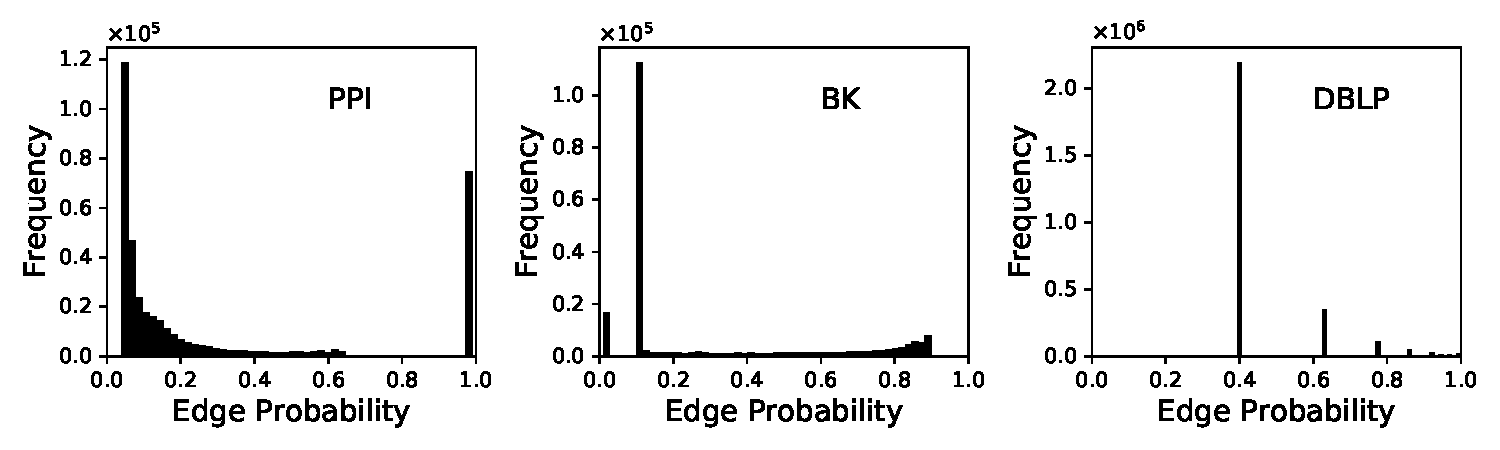
\includegraphics[height=2.6cm]{expResult/probDistribution.pdf}
	\end{flushleft}
	\vspace{-10pt}
	\caption{Edge probability distributions.}
	\vspace{-10pt}
\end{figure}
\begin{figure}[!t]
	\begin{flushleft}
	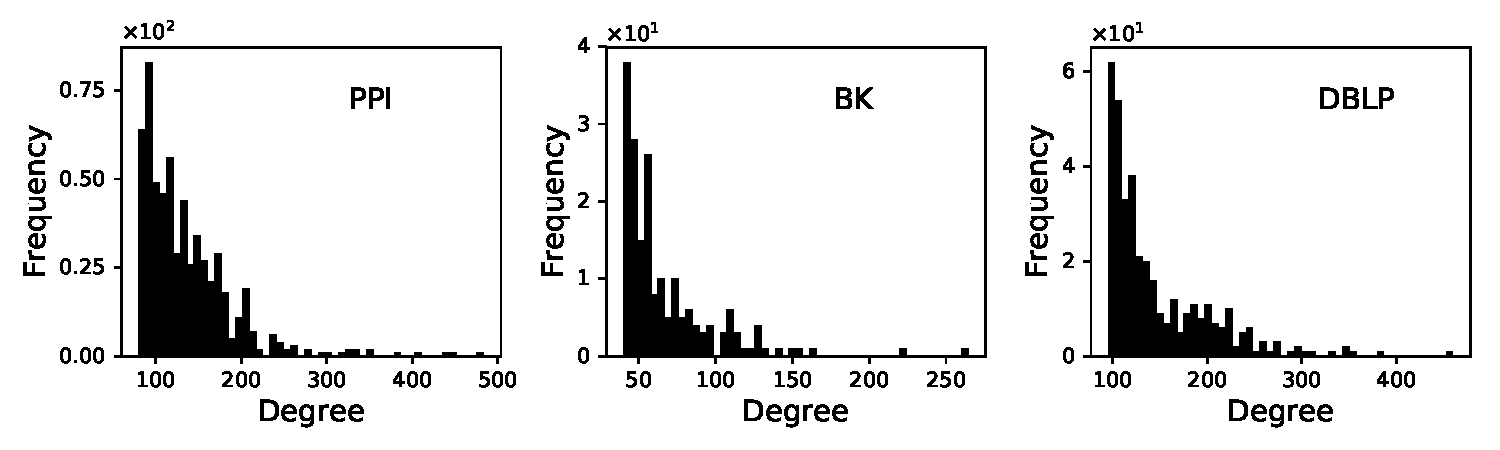
\includegraphics[height=2.6cm]{expResult/degDistribution.pdf}
	\end{flushleft}
	\vspace{-10pt}
	\caption{Degree distributions.}
	\label{fig:degreeDist}
	\vspace{-10pt}
\end{figure}
Note that edge probability values of BrightKite and DBLP are obtained by prediction models built on historical logs which contain sensitive and confidential information. 
These graphs not only capture different real-world scenarios but also different data characteristics {\eg}, size, density, edge probability. 
The graphs size vary from 12K of PPI,  58K of BK, to 824K of DBLP with different densities; 
DBLP is the largest but also the sparest dataset.  
The probability values of PPI and BrightKite are generally very small. 
The PPI dataset has a more uniform probability distribution. While, DBLP dataset only has a few probability values.

We report their degree distributions of “unique” nodes whose obfuscation level is smaller than 300 in Figure~\ref{fig:degreeDist}. Observe that, all the three graphs have a heavy-tailed degree distribution. Namely, they are difficult to be obfuscated.

\textbf{Parameter Setting}~~We consider various obfuscation levels, $k \in \{100,150,200,250,300\}$ and possible tolerance values $\epsilon$ to explore the performance difference. 

\textbf{Statistics}~~For every uncertain graph (obfuscated outputs and original ones), we sampled $N$ possible worlds to compute its statistics of interest. Note that it has been shown that 1000 possible worlds usually suffices to achieve accuracy converge.  Then, we compute the discrepancy of obfuscated outputs against the original one. The smaller discrepancy, the better uncertain graph data utility preserving.



\begin{figure*}[!htb]
    \centering
    \subfigure[PPI]{
    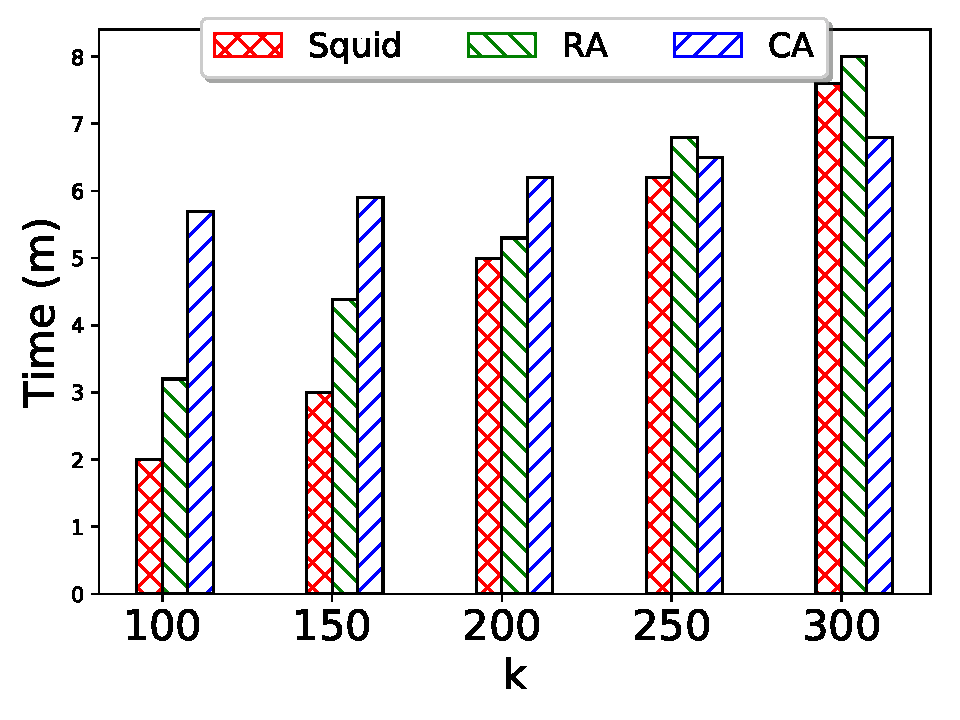
\includegraphics[width=.31\textwidth]{expResult/ppi_time.pdf}
    }
    \subfigure[BK]{
    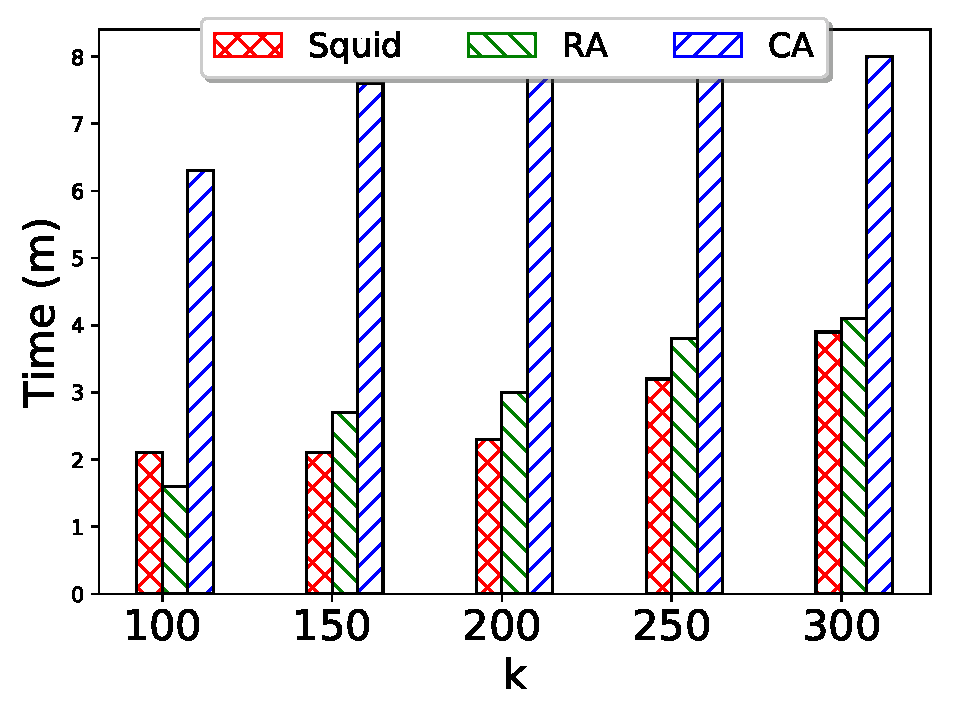
\includegraphics[width=.31\textwidth]{expResult/bk_time.pdf}
    }
    \subfigure[DBLP]{
    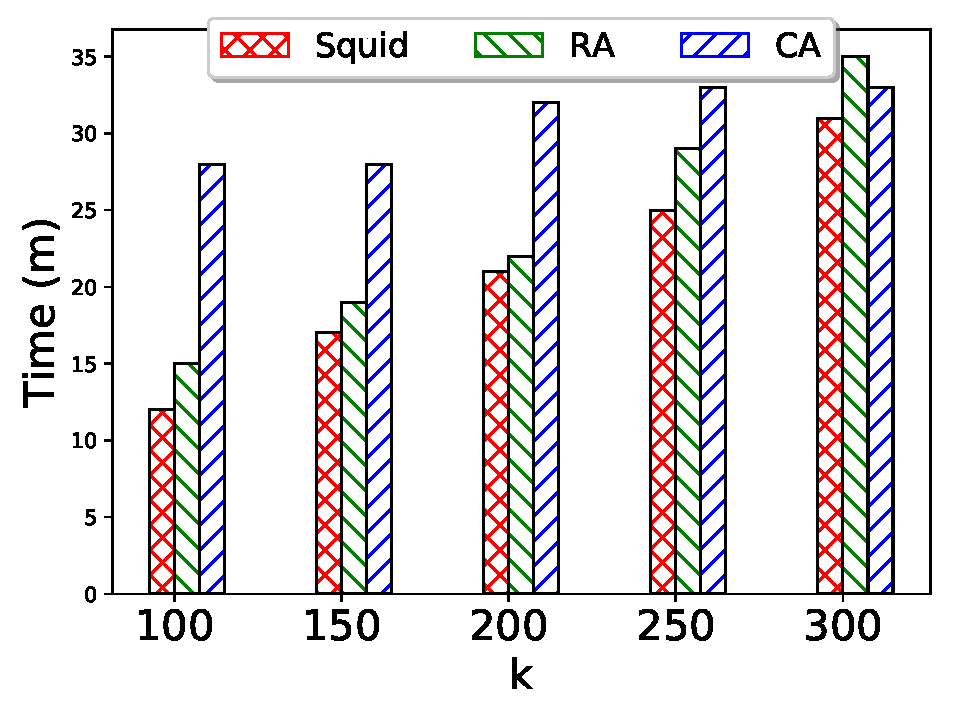
\includegraphics[width=.31\textwidth]{expResult/dblp_time.pdf}
    }
    \vspace{-5pt}
    \caption{Time efficiency of different anonymization methods on three real graphs.}
    \vspace{-5pt}
    \label{fig:time}
\end{figure*} 
\begin{figure*}[t]
    \centering
    \subfigure[PPI]{
    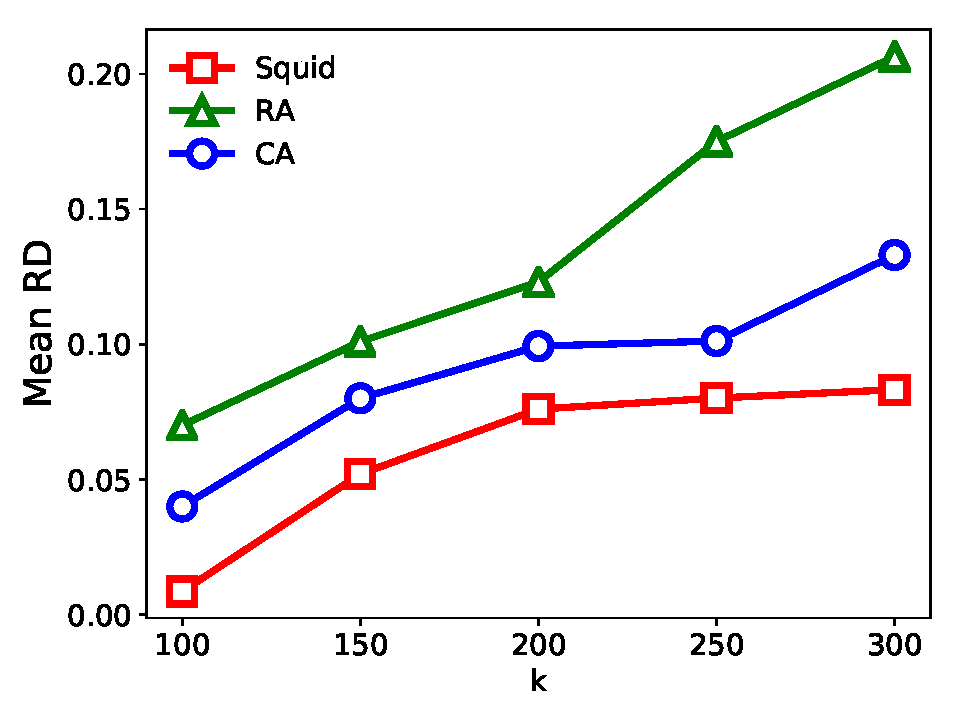
\includegraphics[width=.31\textwidth]{expResult/ppi_RD.pdf}
    }
    \subfigure[BK]{
    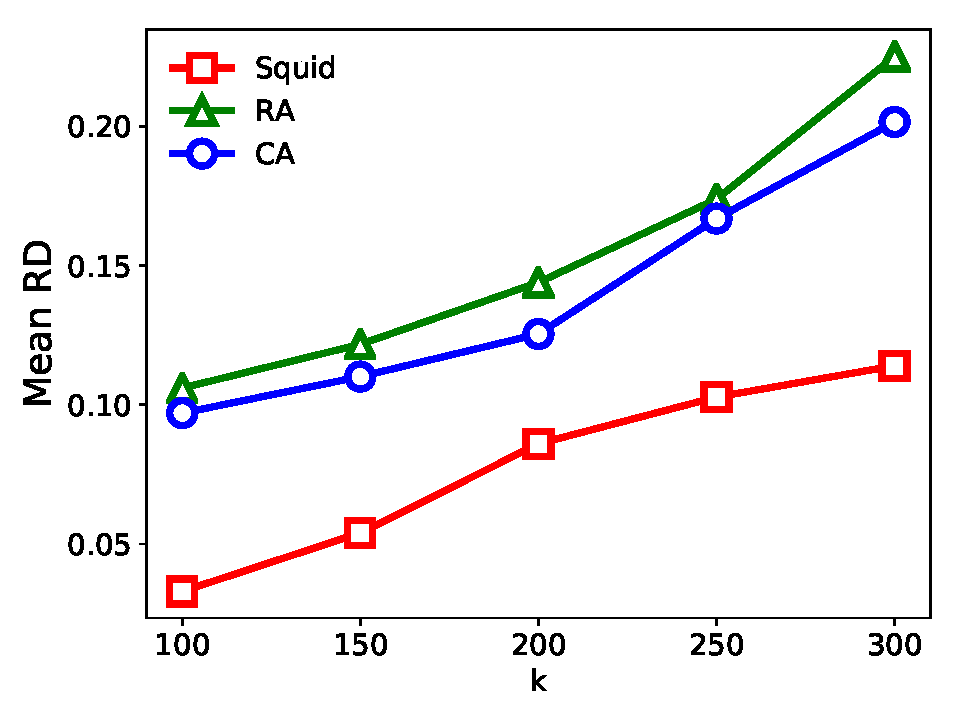
\includegraphics[width=.31\textwidth]{expResult/bk_RD.pdf}
    }
    \subfigure[DBLP]{
    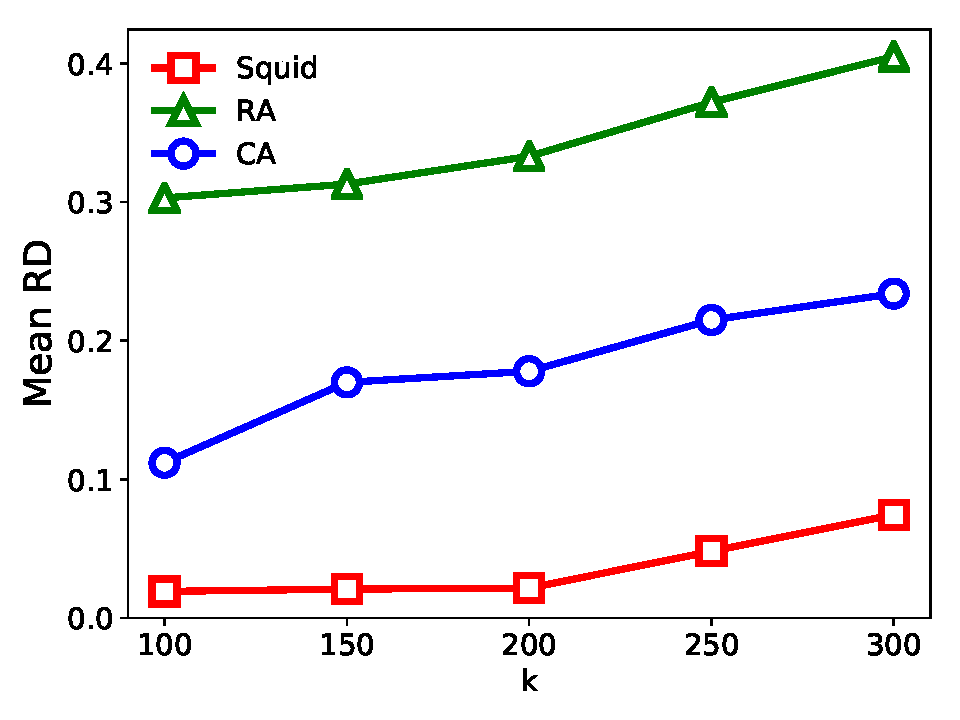
\includegraphics[width=.31\textwidth]{expResult/dblp_RD.pdf}
    }
    \vspace{-5pt}
    \caption{Reliability Discrepancy (RD) of sanitized output graphs of different anonymization methods against original graphs for various values of obfuscation parameter $k$. The smaller the discrepancy the more information of connectivity structure is preserved.}
    \label{fig:rd}
\end{figure*} 
\begin{figure*}[!htb]
    \centering
    \subfigure[PPI]{
    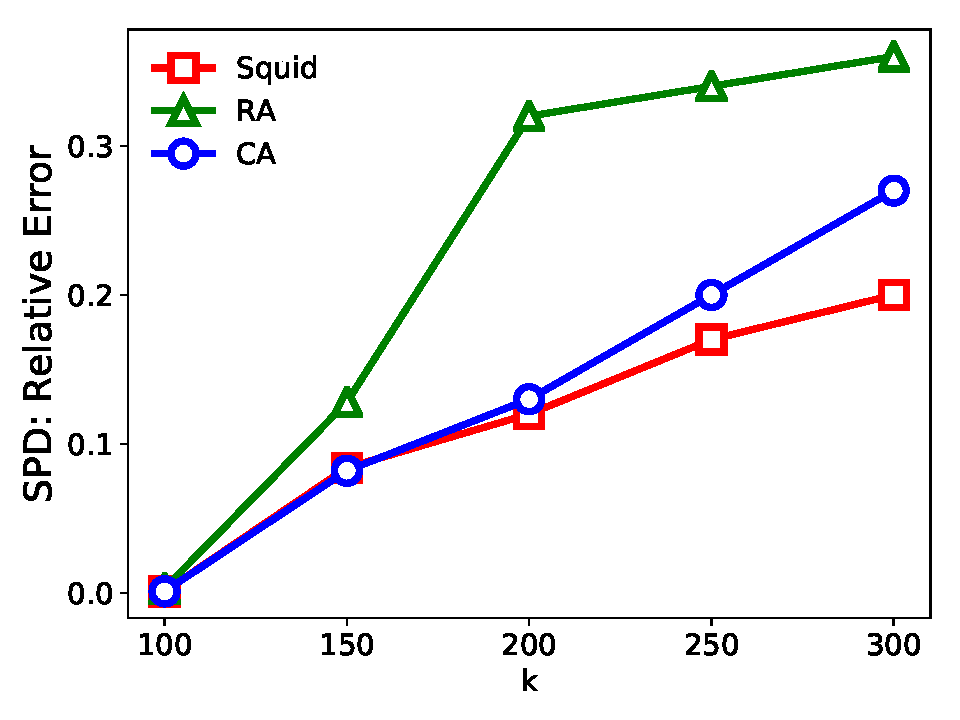
\includegraphics[width=.31\textwidth]{expResult/ppi_PathD.pdf}
    }
    \subfigure[BK]{
    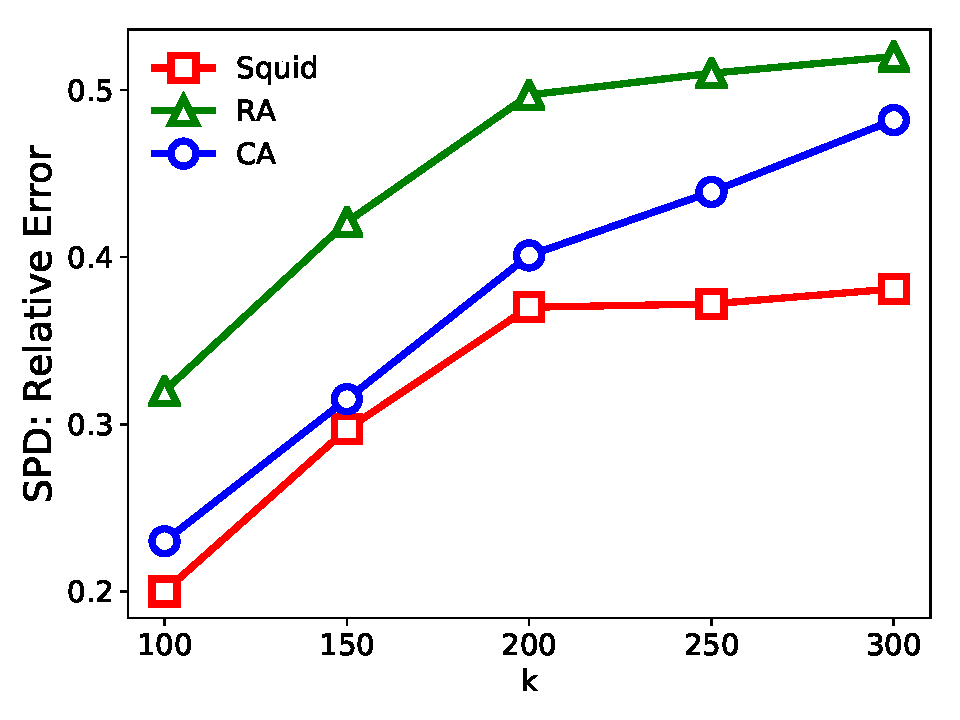
\includegraphics[width=.31\textwidth]{expResult/bk_PathD.pdf}
    }
    \subfigure[DBLP]{
    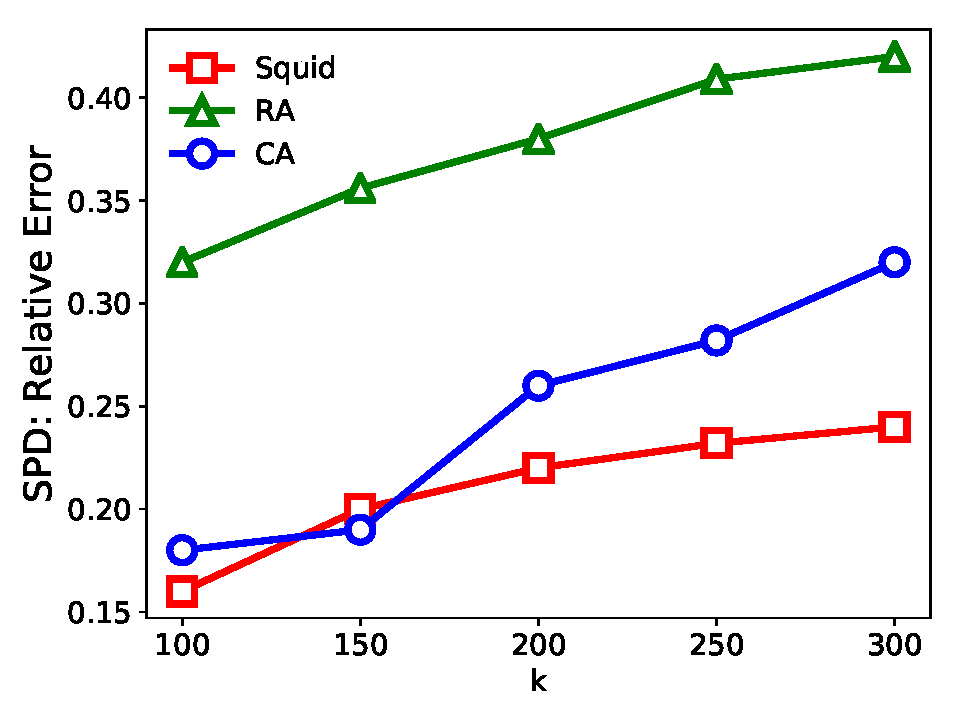
\includegraphics[width=.31\textwidth]{expResult/dblp_PathD.pdf}
    }
    \vspace{-5pt}
    \caption{Relative error of Shortest Path Distance (SPD) of sanitized output graphs of different anonymization methods against original graphs for various values of obfuscation parameter $k$.}
    \label{fig:pathd}
\end{figure*} 

\subsection{Performance Measures}
Three anonymization algorithms were implemented in C++ and run on Intel Core i7 CPU, 2 GHz, 6MB cache size. We measure the time taken for both the pre-processing (representative extraction step in RA) and the synthetic graph generation. 
Figure~\ref{fig:time} shows the time taken to produce sanitized results for PPI, BK, DBLP datasets. 
For larger values for anonymity level $k$, all the methods take more time to find the sanitized solutions. It is because the increased efforts (more noises \& more modified edges) needed to achieve the higher anonymity level (larger values of $k$). 
In summary, our {\methodName} achieves the comparable efficiency with conventional methods.

As shown in Figure~\ref{fig:time}, the time efficiency of our {\methodName} is close to RA, much better than CA in PPI and BK datasets. 
{\methodName} and RA use the same randomized search strategy to identify sanitized solutions using the given standard deviation $\sigma$, while {\methodName} adopts a connectivity model in the probabilistic graph context instead of the degree sequence model adopted in RA. 
Thus, time efficiency depends on how easy it is to find obfuscated solutions that pass the privacy test.  
Note that, the computation of heuristics (generalized uniqueness and reliability relevance) can be finished off-line. 
In the same time, multi-heuristics can co-boost the randomized search strategy in the quite straightforward way with little extra effort. 
Even for severe privacy parameter ({\eg}, $k=300$), Squid can efficiently find obfuscated solutions. 
Meanwhile, CA builds a linear programming (LP) model which preserves properties of weighted graphs are expressible as linear functions of the edge weights. It uses LP solver to find solutions where the computed solutions constitute the weights in the obfuscated graph. 






\begin{figure*}[!htb]
    \centering
    \subfigure[PPI]{
    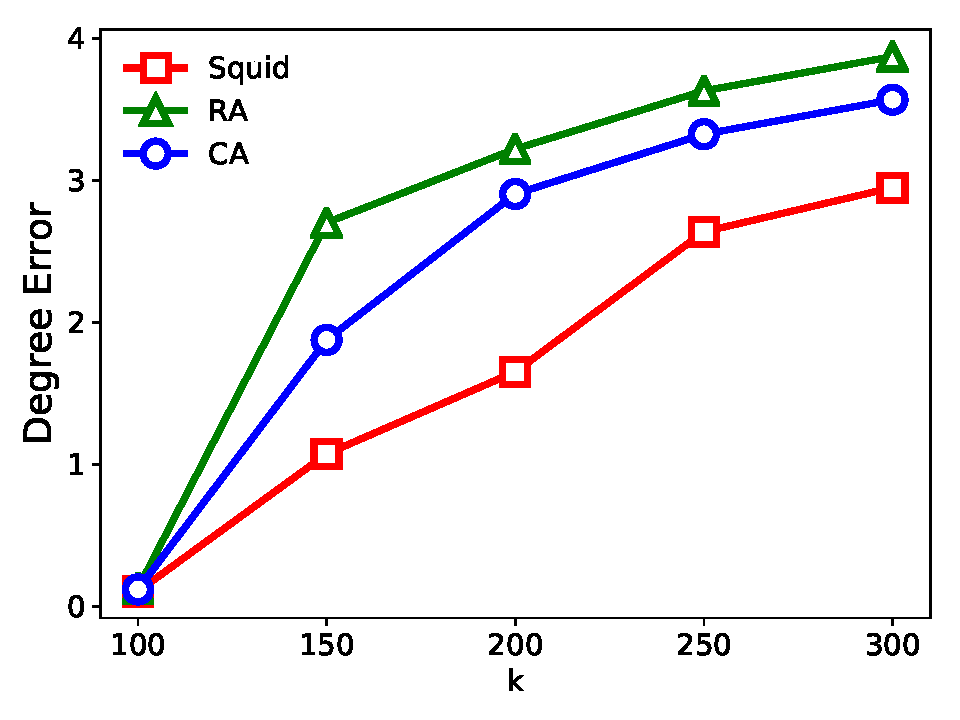
\includegraphics[width=.31\textwidth]{expResult/ppi_dd.pdf}
    }
    \subfigure[BK]{
    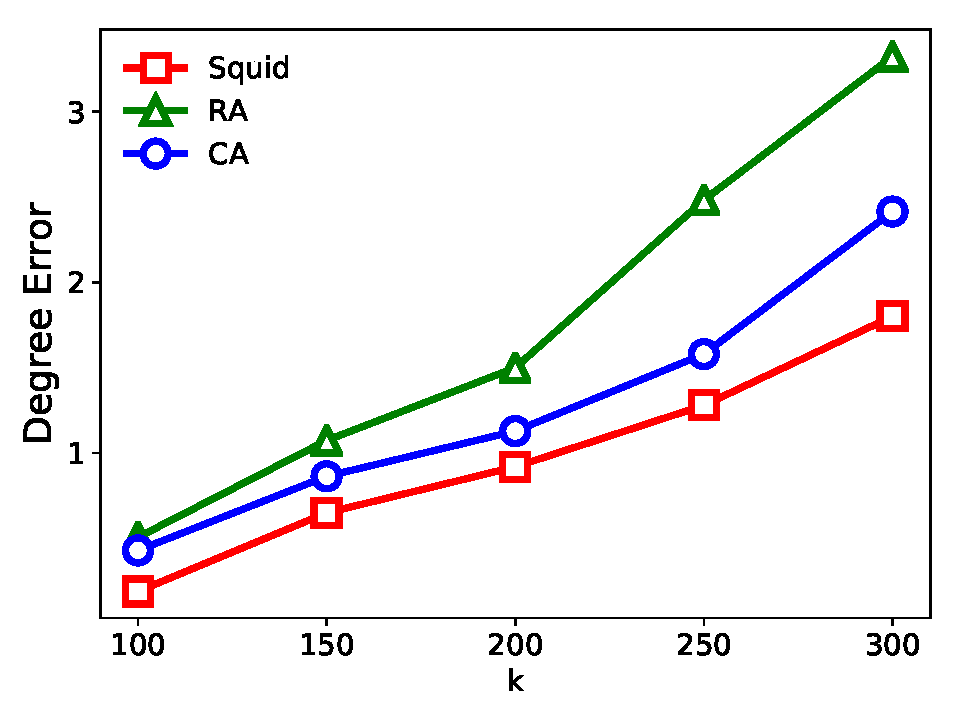
\includegraphics[width=.31\textwidth]{expResult/bk_dd.pdf}
    }
    \subfigure[DBLP]{
    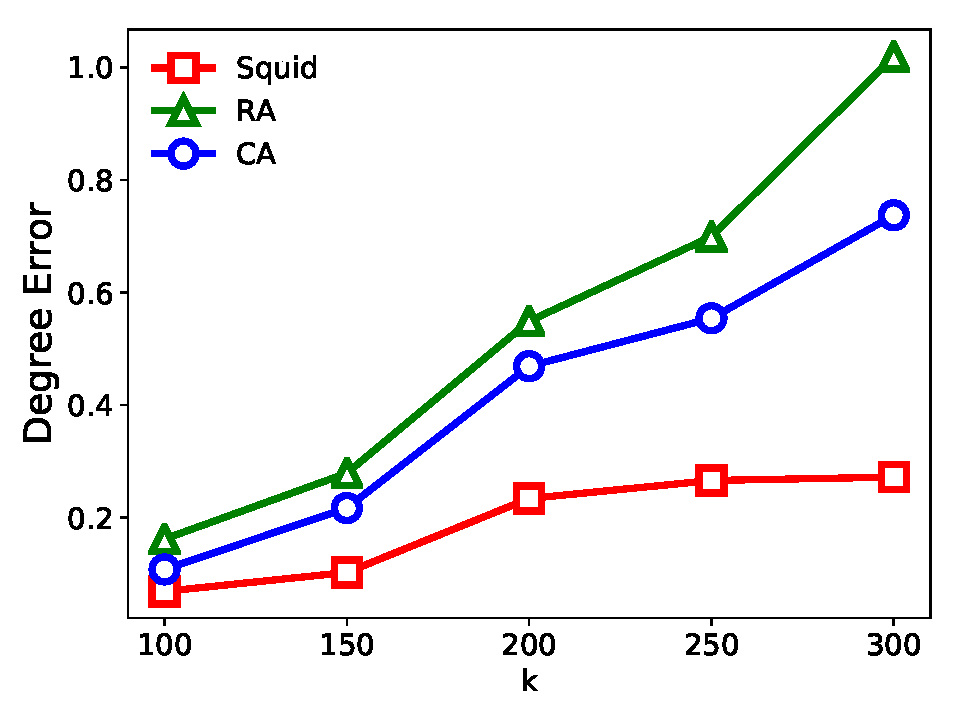
\includegraphics[width=.31\textwidth]{expResult/dblp_dd.pdf}
    }
    \vspace{-5pt}
    \caption{Degree error of sanitized uncertain graphs of different anonymization methods on three real graphs for various values of obfuscation parameter $k$. The smaller the degree error the more information of degree distribution is preserved.}
    \vspace{-5pt}
    \label{fig:dd}
\end{figure*} 
\subsection{Uncertain Graph Statistic Preserving}
In the set of experiment, we focus on evaluating their performance concerning graph statistic preserving. 
The evaluation includes two groups of graph statistics. 
The first group includes node separation statistics that quantify the interconnectivity and density of the overall graph.   
This group includes metrics such as Shortest Path Length, Reliability and Graph Diameter. 
They are very expensive because they involve all-pairs shortest path computations. 
To overcome this problem, we use Hyper ANF~\cite{Boldi_Rosa_Vigna_2011} to approximate shortest path-based statistics.
The second group includes degree-based statistics such as Average  Node Degree and Degree Distribution.
These topological statistics that characterize how degrees are distributed among nodes. 
Our results are highly consistent across our pool of graph statistics.
For brevity, we only report  Reliability, Shortest Path Length and Node Degree as their representatives. 

\textbf{Node Separation Statistic.} 
Figure~\ref{fig:rd} shows the incurred reliability discrepancy. 
We can see that larger $k$ introduced more significant connectivity distortion due to the fact that more noise was added to achieve the desired level of anonymity.   
These observations are consistent across biological (PPI) and social  networks (BK and DBLP).

{\methodName} method preserves very well reliability in all datasets, followed by the CA approach with the similar objective function. RA performs poorly for DBLP. 
For example, in all the dataset ($k=300$), the reliability discrepancy introduced by {\methodName} is well below 0.1 whereas the ones added by CA is below 0.2. The reliability discrepancy introduced by RA on PPI, BK, DBLP is around 0.2, 0.2, 0.4 respectively. We also observe that as the size of graph increases (PPI $\rightarrow$ DBLP), the performance gap becomes larger and larger.

Note that CA and RA schemes deteriorate data utility due to the disregarding the possible world semantics. 
For example, in the case, $k=100$ (weak privacy guarantee required little noise), CA and RA incur relatively large connectivity distortion.  
The representative extraction step of RA introduces noise and results in cumulative errors in the anonymization step. Consequently, sanitized results differ from the original ones. 
The CA scheme fails to reflect the connectivity of uncertain graph correctly. Thus, it produces inferior results even with the similar objective function.  

Figure~\ref{fig:pathd} shows the relative error of \emph{Shortest Path Distance} of sanitized output graphs. In general, the ranking of anonymization algorithms regarding preserving path-based statistic is analogous to that for reliability (see Figure~\ref{fig:rd}) because the shortest path distance between a node pair $\langle u,v\rangle$ is highly correlated to two-terminal reliability. 



\textbf{Degree-based Statistic.}~Figure~\ref{fig:dd} shows the error of Node Degree values on PPI, BK and DBLP compared to their sanitized outputs. 
The obfuscated output of {\methodName}, CA capture well Node Degree in all datasets; 
our method {\methodName} is consistently better.    
In the largest dataset DBLP, the degree error $0.2$ is much lower than $1.08$ imposed by the two-phase anonymization scheme (RA) in the same level of obfuscation ($k=300$).  
As with previous experiments, the performance gap increases as the graph size increases.

\textbf{Summary.} 
Our experimental results show that sanitized outputs generated by {\methodName} exhibit structural features close to those of their original uncertain graphs. 
Results show that we can effectively balance the utility and privacy in the probabilistic graph context.
The result is encouraging because we can eliminate the noise by moving from the reliability model to a more accurate graph model incorporating with the possible world semantics.
\subsection{Application Results}
\begin{figure}[!htb]
    \centering
    \subfigure[PPI]{
    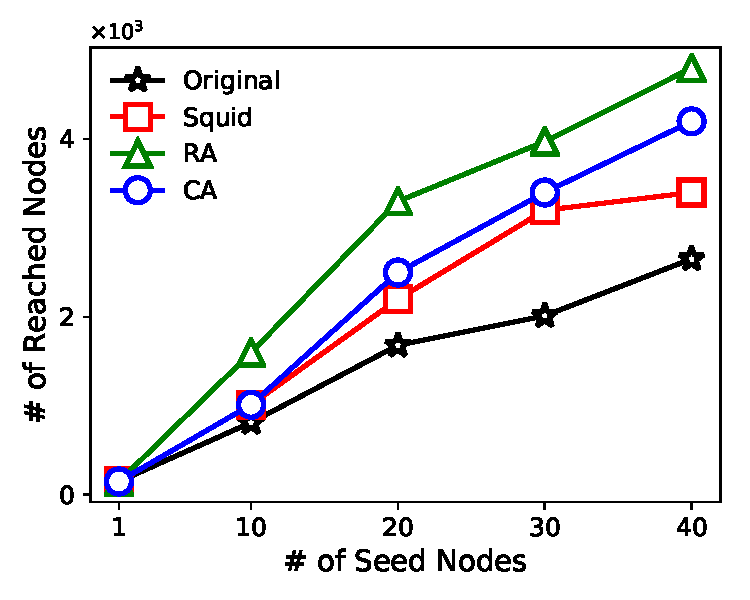
\includegraphics[height=3cm]{expResult/ppi_IM.pdf}
    }
    \subfigure[BK]{
    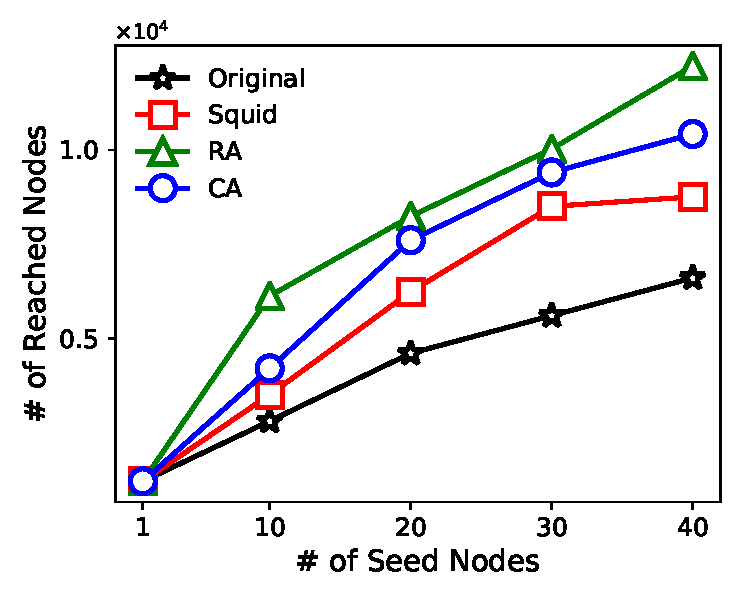
\includegraphics[height=3cm]{expResult/bk_IM.pdf}
    }
    \caption{Results of the Degree Discount Influence Maximization algorithm on PPI, BK datasets, 
    compared to sanitized graphs where $k$=100.}
    \vspace{-10pt}
    \label{fig:IM}
\end{figure} 
For a sanitized graph to be meaningful for research use, it should produce 
the close results as the original graph in the application-level settings. 
Influence Maximization is known as essential techniques with advertisement and public relation campaigns.
It tries to locate users in the network who can most quickly spread influence through the network. 
Usually, related algorithms start with identifying the nodes which can maximize influence and model the spread of influence through network how many users has ultimately reached.  
Motivated by these facts, we compare the result of influence maximization on sanitized outputs and original graphs. 
In general, it enables us to quantify the trade-off between application utility and privacy protection. 

\textbf{Methodology.}~~Since there do not exist closed formula for the number of influenced nodes, we approximated the expectation value of influence by Monte Carlo Sampling. We create a number of random instance of the uncertain graph. For each sampled graph, we adopt the degree discount method (a heuristic-based method with light computation) to find the most influential nodes (seeds) on a deterministic graph. Starting from those seeds, we run the weighted cascade influence dissemination model to determine the number of reached users in the network. 

For the limit of computation resource (memory overhead), we only perform the set of experiment over PPI and BK datasets. We report the expected number of reached nodes when the number of initial seeds in Figure~\ref{fig:IM}. 
There are clear and visible trends across PPI and BK datasets. 
Graphs with privacy protection diverge from the results of original graphs.
We found that our method {\methodName} excelled in preserving the information propagation pattern, followed by CA that aim explicitly at preserving linear property. Similar to previous experiments, RA performs poorly due to the erroneous measurement of the impact on structural integrity from anonymization process.  

Overall, our experimental assessment on influence maximization applications confirms our intuition: by incorporating the possible world semantics into the core of anonymization, one can achieve the same desired level of anonymity with a smaller impact in the uncertain graph utility.  

\section{Conclusion}
In this work, we first examine the overlooked problem of privacy-preserving uncertain graph sharing. 
We provide a generalized scheme, {\methodName}, which seamlessly integrates edge uncertainty into core anonymization steps.
The scheme uses a randomized algorithm boosted by the hybrid of utility-aware heuristics. 
It excels in identifying sanitized uncertain graphs with excellent quality. 
Experiments on three real-world datasets verify its effectiveness and practical utility.
There are many potentials to explore further.  
The independent model discussed in this work is one of the simplest models with uncertainty, it naturally ignores the correlation among various graph components. 
We leave the conditional probability model as a future extension. 
Another extension is to investigate sharing uncertain graphs in the differentially private manner.

\bibliographystyle{ACM-Reference-Format}
\bibliography{refs} 

\end{document}
